% Use only LaTeX2e, calling the article.cls class and 12-point type.

\documentclass[11pt]{article}
\usepackage[table]{xcolor}% http://ctan.org/pkg/xcolor
\usepackage{times}
\usepackage{graphicx}
\graphicspath{{figures/}} %Setting the graphicspath
\usepackage{caption}
\usepackage{subcaption}
\usepackage{enumitem}
\usepackage{multirow}

%\usepackage{breakurl}
%\usepackage{url}
%%% --- The following two lines are what needs to be added --- %%%
%\setcounter{biburllcpenalty}{7000}
%\setcounter{biburlucpenalty}{8000}

\usepackage{color}   %May be necessary if you want to color links

%\usepackage[hyphens]{url}
\usepackage{hyperref}
%\PassOptionsToPackage{hyphens}{url}\usepackage{hyperref}

\hypersetup{
	%hidelinks, % Remove visible links altogether
	%urlbordercolor = 1 1 1, % Make URL link border white
	breaklinks=true,
    colorlinks=true, %set true if you want colored links
    linktoc=all,     %set to all if you want both sections and subsections linked
    linkcolor=blue,  %choose some color if you want links to stand out
}   

\usepackage{setspace}

% The following parameters seem to provide a reasonable page setup.

\topmargin 0.0cm
\oddsidemargin 0.2cm
\textwidth 16cm 
\textheight 21cm %21cm
\footskip 1.0cm %1.0cm


\renewcommand\refname{References and Notes}

\newcounter{lastnote}
\newenvironment{scilastnote}{%
\setcounter{lastnote}{\value{enumiv}}%
\addtocounter{lastnote}{+1}%
\begin{list}%
{\arabic{lastnote}.}
{\setlength{\leftmargin}{.22in}}
{\setlength{\labelsep}{.5em}}}
{\end{list}}


\begin{document} 

% Double-space the manuscript.

% Include your paper's title here

\title{Prediction of Scores for Public Schools in California}

\author
{Ahrim Han, Ph.D.\\
\\
}

% Include the date command, but leave its argument blank.

\date{June 15, 2019}



%%%%%%%%%%%%%%%%% END OF PREAMBLE %%%%%%%%%%%%%%%%

% Make the title.

\maketitle 
\newpage

\doublespacing
\tableofcontents
\singlespacing
\newpage

\baselineskip24pt

\section{Introduction}

\paragraph*{Problem Statment.}

The California Assessment of Student Performance and Progress (CAASPP) is the assessment system to measure how well students are mastering California’s academic standards in English language arts/literacy and mathematics. These results can be used to monitor the student progress and to give feedback the teachers need to change teaching methods more effectively. However, the test scores vary widely from school to school. There is a common belief that affects high test scores such as \textit{schools with many Asian students} or \textit{schools with high-income families}. There is a strong need to find more informed and granular causes that impact the test achievements of schools. 
%
Ultimately, \textbf{we aim to predict and find the inferior groups of schools that indeed need help}. I suggest the expected beneficiaries with the provided results.

\paragraph*{Expected Beneficiaries.}

\begin{itemize}
\item To broadening educational opportunities, administrators of the school districts/state departments of education or other organizations can effectively identify the schools that need most supports. Budgets and human resources can be allocated in the order of the needs for tutoring, mentoring, extracurricular programs, educational consultants, and so on. In the equity aspect, schools should strive to create an environment where all students feel valued and all students are learning to high standards. 
\item Teachers can put much more effort into the under-performing groups to reduce the achievement gaps. 
\item From a parent’s perspective, these results can be an indicator to select a good school that meets the high academic standards.
\end{itemize}

\paragraph*{Approach.}

We acquired the CAASPP test score data in 2018 from the California Department of Education \cite{california_dep_education, california_dep_education_caaspp, CAASPP_research}. 
%\url{https://caaspp.cde.ca.gov/}.
%for years from 2015 and 2018 (5 years).
%%teacher demographics [3] 
In data wrangling (Section \ref{Data Wrangling}), we performed data cleaning, fixing missing values, and adding new columns.
%
For obtaining more meaningful analysis results and building a more accurate prediction models, we combined the information on median house prices \cite{Zillow_research_data, Civil_Rights_Data_Collection}. 
%
Missing values are imputed using the statistics of the \textit{mean} of each column in which the missing values are located.
%
We basically divide
the percentage of the students 
into four achievement groups ‘Standard Exceeded (Level 4)’, ‘Standard Met (Level 3)’, ‘Standard Nearly Met (Level 2)’, ‘Standard Not Met (Level 1)’ and focus to predict the top (Level 4) or bottom (Level 1) groups.

%
In the data visualization (Section \ref{Data Visualization}) and exploratory data analysis (Section \ref{Exploratory Data Analysis}), we plotted the various kinds of graphs (including \href{https://github.com/ahrimhan/data-science-project/blob/master/project1/data_visualization.ipynb}{interactive stacked bars using Plotly library}) and gained the insights on \textbf{exceeded scores} and \textbf{inferior scores} regarding to \textbf{gender, ethnicity, english-language fluency, economic status, disability status, and parent educations}.
%
We also performed correlation analysis, univariate selection, and feature importance methods to find the strong indicators affecting lower scores. 


%machine learning
In the modeling (Section \ref{Modeling}), we used the supervised machine learning  algorithms including the regression and classification to build predictive models. 
%
The regression algorithm predicts the percentage of students who do not meet the standard. The classification algorithm predicts if the schools ``need help" (1) or "do not need help" (0). 
%
We set the ``need help" schools that has more than ``80\% of the standard not met" students (312 out of 8,786 schools).
%
We tried various machine learning techniques to pick the one which performs best.
%
For regression, out of 5 different models, we obtained the best regression model using the random forest regressor with 10 folds cross validation
with the accuracy of RMSE 10.77, MAE 7.69, and R$^{2}$ 0.68.
%
For classification, we tried to solve the class imbalanced problems using the Stratified K-fold cross validation and the weighted evaluation metrics to reflect the mass of the classes. In addition, we scaled the training data and significantly improved the accuracy of the K-Nearest Neighbor algorithm.
%
As a result, we obtained the best classification model using the random forest classifier based on grid search cross validation with the accuracy 0.97 and AUC 0.98.
%We obtained the best classification model with the accuracy 0.97 and the AUC 0.97 using the random forest classifier with grid search cross validation using the three parameters each of three values. 

%Recommendations
Based on these results, we identified the top and bottom schools and found the important features determining those schools.
%
We recommended some strategies
that effectively increase the achievements for scores in Section \ref{Limitation and Recommendation}. 


\section{Data Wrangling} \label{Data Wrangling}

In this section, we perform data cleaning, fix missing values, and add
new columns with meaning values. 
More details with codes on data wrangling can be found in
\href{https://github.com/ahrimhan/data-science-project/blob/master/project1/data_wrangling.ipynb}{this IPython notebook}. 


\subsection{Data Loading and Manipulating}

\subsubsection{CAASPP Test Scores}
%\url{https://caaspp.cde.ca.gov/}.
%for years from 2015 and 2018 (5 years).
The test type is the Smarter Balanced Assessment Consortium (SBAC) of English Language Arts/Literacy and Mathematics.
The data set is too large to commit to GitHub, we uploaded the data in our space. You can download the data here \cite{CAASPP_download}.
Besides the CAASPP test scores, \textbf{Test data file},
the information is separated into 3 files, 
\textbf{Entity table, Subgroup ID table, and Test Id table},
so that these files must be merged with the test data file to join the names with the appropriate score data.

%\paragraph*{Test data file.}
\begin{itemize}
\item
  The public score data is available between 2015 and 2018 (4 years)  \cite{california_dep_education, california_dep_education_caaspp, CAASPP_research}. We only used data in the year of 2018. 
\item 
For each year data, the test data file is provided in a `csv file' format. For the record of 2018, for example, there are 3,269,730 rows with 32 columns.
\item 
This data contains the scores of two parts, English Language Arts (ELA) and Mathematics, for students in grades 3-8 and grade 11. The test data is comprised of state, counties, districts, and schools along with the test scores. The information on parent education, races, disabilities, gender, English-Language fluency can be combined with the test data. 
\end{itemize}

The data was imported into DataFrame of Pandas. I decided to use only the next columns: `Country Code', `District Code', `School Code', `Test Year', `Subgroup ID', `Grade', `Test Id', `Students with Scores', and achievement levels. The minimum and maximum test scale score ranges are provided here \cite{score_range}. The `Mean Scale Score' is used to determine four achievement levels: 
%
\textbf{‘Percentage Standard Exceeded’, ‘Percentage Standard Met’, ‘Percentage Standard Nearly Met’, ‘Percentage Standard Not Met’}. Many studies showed that discretization can lead to improved predictive accuracy and is more understandable \cite{Discretization}.

The test score data also has area descriptors \cite{CAASPP_understanding}. There are 4 areas of reading, writing, listening, and research/inquiry for ELA whereas 3 areas of concepts and procedures, problem solving/modeling and data analysis, and communicating reasoning for mathematics. For each area, the achievement levels are divided into ‘Above Standard’, ‘Near Standard’, and ‘Below Standard’ depending on the scale scores compared to the ‘Standard Met’ achievement level on the total content-area test.

The \textbf{Entity table} lists the County, District, and School entity names and codes for all entities as the existed in the administration year selected. This file must be merged with the test data file to join these entity names with the appropriate score data.

Here are detailed explanations and decisions made toward the data.

\begin{itemize}
\item
To evaluate school performance, we use the four achievement levels instead of ‘Mean Scale Score’. The levels are about intervals of numbers which are more concise to represent and specify, easier to use and comprehend as they are closer to a knowledge-level representation than continuous values. 
\item
The ‘Grade’ represent 3-6 grades (elementary schools), 7-8 grades (middle schools), and 11 grade (high schools). The ‘Grade’ 13 denotes all grades \cite{CAASPP_Research}, so we decided to use data only 13 for minimum sample size. I believe the aggregated data at each school level is enough for representing the characteristics of public schools in California.
\item
The \textbf{Subgroup ID} lists the codes with the groups (e.g., gender, English-language fluency, economic status, ethnicity, (ethnicity for economically disadvantaged, ethnicity for not economically disadvantaged), disability status, parent education, migrant). 
\item
The \textbf{Test Id} is 1-4; 1 represents ELA and 2 represents mathematics, respectively. We only consider ‘Test Id’ 1 and 2. The ‘Test Id’ 3 and 4 are excluded because they are CAA (California Alternative Assessments) scores. The CAA scores are taken by students in grades 3–8 and grade 11 whose individualized education program (IEP) teams have determined that the student's cognitive disabilities prevent him or her from taking the online CAASPP Smarter Balanced assessments.
\end{itemize}

\subsubsection{House Price}

The Zillow Home Value Index (ZHVI) data \cite{Zillow_research_data} was imported and loaded. The ZHVI is a seasonally adjusted measure of the median estimated home value across a given region and housing type. The data was collected from April 1996 to November 2018 on monthly basis. I cleaned up the data by dropping house prices that are less than 2018. To analyze the school performance on a yearly basis, \textbf{the monthly prices were grouped by each year into a median value}.

I had tried two different versions when dealing with time data: data manipulation using 1) \texttt{DatetimeIndex} objects and 2) using user-defined functions. I found the first method is more convenient and safe for dealing with time related data. For example, even though I assured to use years as an \texttt{int64} type, it may cause unexpected spaces to be inserted. However, this can cause errors because when merging data tables requires keywords of the same data type. Therefore, we first manipulate the time data using \texttt{DatetimeIndex} objects, and then finally, we
convert columns of `Test Year' from \texttt{DatetimeIndex} to \texttt{int64} for compatibility.


\subsection{Joining Multiple Datasets and Cleaning Data}
There are multiple dataset and we need to merge efficiently to obtain useful and clean data. The diagram in Figure 1 shows multiple data and merging keys among them. 
To obtain the test scores of specific schools, districts, or counties, we first should get the exact school codes from entity tables. When finding the school codes, you should specify a county, a district, and a school names because there may exist several schools with the same names. These are denoted as the ‘CDS’. Please note that if we specify only the school name(s), we could retrieve the several schools with the same names. It is important to include these three codes to avoid the double-counting in any summary calculations.
Using the CDS codes, we then retrieve the DataFrame of the test data scores of a school. In the same way, we can retrieve the DataFrames of the county and the district. We append the specific names to the test score DataFrame by merging two tables (Test data + entities). We dropped the columns ‘Type Id’ and ‘Test Type’ since they are not have significant meanings as school performance indicators.
At last, we merge the house prices and test score data. 
%We finally obtain the clean data.

\subsection{Detecting and Imputing Missing Values}

\paragraph*{Detecting missing values.} 

Many of the data of Subgroup ID are missing. In the test scores, the missing data is filled with some symbols (e.g., ‘*’ and ‘-’). Thus, even DataFrame.info() function retrieves as all data are existed, we need to substitute these symbols as NaN (missing data).

A basic strategy to use incomplete datasets is to discard entire rows and/or columns containing missing values. However, this comes at the price of losing data which may be valuable (even though incomplete).  
%We notice that only score columns have the missing values, and the number of missing values for every score column are same. This means that one row has all missing scores or all scores.
So, we first \textbf{drop the 252,877 rows having NaN in all scores}.

\paragraph*{Imputing for missing values.}

Before we put features into a model, missing values must be filled and all features must be encoded.
%For various reasons, many real world datasets contain missing values, often encoded as blanks, NaNs or other placeholders. 
Datasets such as blanks, NaNs or other placeholders are incompatible with \textit{scikit-learn} estimators which assume that all values in an array are numerical, and that all have and hold meaning. 
A good strategy is to impute the missing values, i.e., to infer them from the known part of the data (\url{https://scikit-learn.org/stable/modules/impute.html}).
%
To deal with the missing values, we use the basic strategies for imputing missing values. \textbf{Missing values are imputed using the statistics of the \textit{mean} of each column} in which the missing values are located.

Finally, we also drop the schools containing names of ``Program" and ``Alternative".
Then, we preliminarily finalize our data at this stage.

\section{Data Visualization}
\label{Data Visualization}

In this section, we explored the data to find trends, correlations, insights, and potential outliers based on visualization.
These graphs and figures are important as a communication tool
for collaborating in data science teams or 
presenting to business-oriented customers.
%
For utilizing advanced features, we used the \textbf{seaborn and Plotly libraries} in addition to \textbf{Matplotlib library}.
In this California score data, there are 52 counties, 784 districts, and 6,539 schools.
%
Please note that the data is \textbf{grouped by County levels}.
Before building a prediction model in school-level, it is worth to find rough trends in the bigger level such as the counties rather than the levels of districts or schools. 
%
More details with codes on data visualization can be found in
\href{https://github.com/ahrimhan/data-science-project/blob/master/project1/data_visualization.ipynb}{this IPython notebook}. 


\paragraph{Hypothesis.}
We start with the following hypothesis.
\begin{itemize}
\item The schools with many Asian students tend to achieve high scores.
\item The schools with high-income families tend to achieve high scores.
\item The schools with highly educated parents tend to achieve high scores.
\item The schools surrounded by high house costs tend to achieve high scores.
\end{itemize}

\paragraph{Research Questions.}
Therefore, we investigate the following three research questions.
\begin{enumerate}
	\item How students are different in achievement levels for each category? (Section \ref{Comparison for All Students Using Bar Plot})
\item What features can you find in the top and bottom performance groups? (Section \ref{Comparison for Top and Low Performance Groups Using Bar Plots})
\item Are house prices correlated to the exceeded scores or the inferior scores?
(Section \ref{Correlations Using Scatterplots})
\end{enumerate}


\subsection{Comparison of Scores in Each Student Category Using Bar Plots}
\label{Comparison for All Students Using Bar Plot}

We provide two different version of bar plots for each category---\textit{all four achievement levels in a stacked bar} and \textit{specific achievement levels in a parallelized bar}.

\subsubsection{Gender}
\textbf{Figure \ref{fig:all_gender} shows that female students exceed male students in English, while male students exceed female students in Mathematics.}
\begin{itemize}
	\item In the English subject at the "Standard Exceeded" level, females students are 6.4\% more than males students.
\item In the mathematics subject at the "Standard Exceeded" level, males students are 1.4\% more than female students.
\item At the "Standard Met" above level ("Standard Exceeded" + "Standard Met"), females students are 10.8\% more than males students in English (females: 50.9\% $>$ males: 40.1\%). In mathematics, there are not much difference (males: 34.8\% $>$ females: 34.6\%).
\item \textbf{The subject difference of female students is much bigger than male students.}  At the "Standard Met" above level , female students are 16.3\% more in English than in mathematics. In contrast, the males students are 5.3\% more in English than in mathematics.  
\end{itemize}


%https://www.latex-tutorial.com/tutorials/figures/
\begin{figure}[h!]
\centering
\begin{subfigure}{0.35\textwidth}
         \centering
         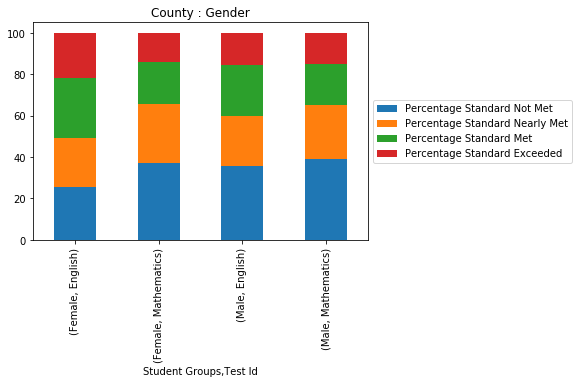
\includegraphics[width=\textwidth]{output_24_0.png}
         \caption{All achievement levels}
         \label{fig:gender_all}
\end{subfigure}
\hfill
\begin{subfigure}{0.6\textwidth}
         \centering
         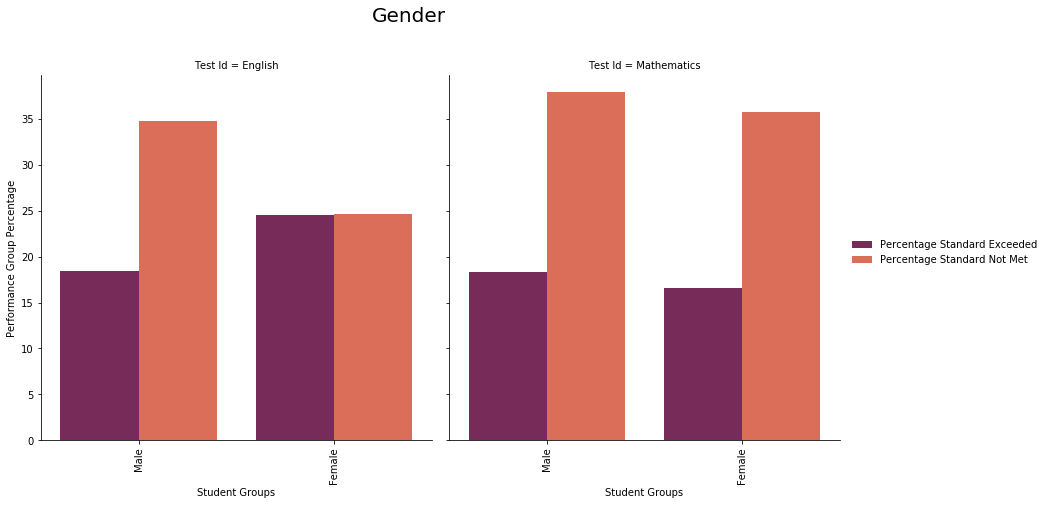
\includegraphics[width=\textwidth]{output_26_1.png}
         \caption{Comparison of highest and lowest achievement levels 
in English and Mathematics}
         \label{fig:gender_two}
\end{subfigure}
\caption{Bar plots for gender.}
\label{fig:all_gender}
\end{figure}

\subsubsection{Ethnicity}
\textbf{Figure \ref{fig:all_Ethnicity} shows that Asian students achieve the best performance, while Black or African American and American Indian or Alaska Native students achieve the lowest performance in both English and mathematics.}

\begin{itemize}
	\item \textbf{Students' achievements are higher} (there are the most "Standard Exceeded" students) in the order of Asian, Filipino, two or more races, and white, for both English and mathematics.
\item \textbf{Students' achievements are lower} (there are the most "Standard Not Met" students) in the order of Black or African American, American Indian or Alaska Native, Native Hawaiian or Pacific Islander, and Hispanic or Latino in both English and mathematics.
\item \textbf{The ethnic group of students in the "Standard Not Met" level has much more difficulties in mathematics} than English. 
\end{itemize}
  
\begin{figure}[h!]
\centering
\begin{subfigure}[h]{0.35\textwidth}
         \centering
         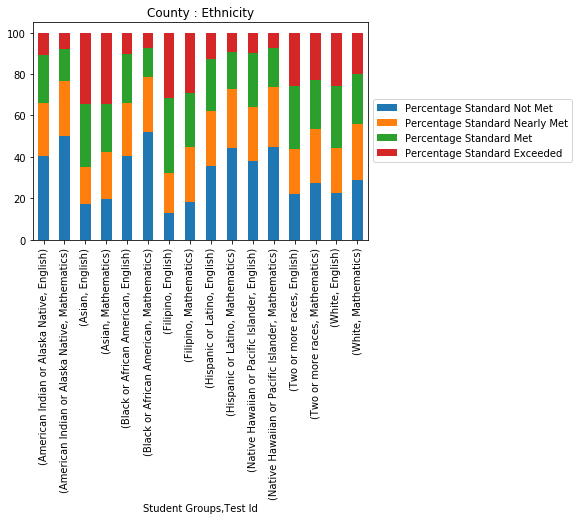
\includegraphics[width=\textwidth]{output_28_0.png}
         \caption{All achievement levels}
         \label{fig:Ethnicity_all}
\end{subfigure}
\hfill
\begin{subfigure}{0.6\textwidth}
         \centering
         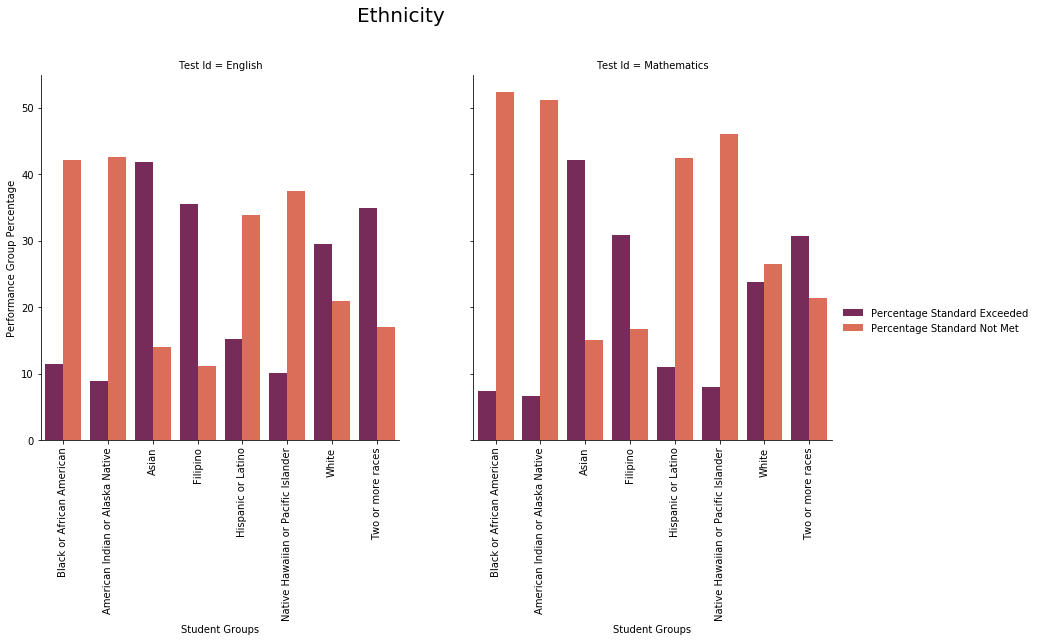
\includegraphics[width=\textwidth]{output_29_1.png}
         \caption{Comparison of highest and lowest achievement levels 
in English and Mathematics}
         \label{fig:Ethnicity_two}
\end{subfigure}
\caption{Bar plots for ethnicity.}
\label{fig:all_Ethnicity}
\end{figure}

\paragraph{Ethnicity Distribution for Top and Bottom Scores.}
We further analyze the distribution of four ethnicity groups (i.e,. Asian, Whites, Black, and Hispanic students) 
distributed in top scores (``Percentage Standard Exceeded") and bottom scores (``Percentage Standard Not Met").

Figure \ref{fig:Ethnicity_distribution} shows that Asian students are in the diverse range of the percentage of high scores. In short, many of the Asian students exceeded in some schools but a small portion of Asian students exceeded in other schools.

However, there are a few Black and Hispanic students who achieve the exceeded standard scores. As you can see, the graphs in the Black and Hispanic distribution, the graph bar is skewed to the left. This means that a small portion of Black and Hispanic students exceeded some other schools, but there is almost no counts that the majority or a high portion of those Black and Hispanic students achieve the high performances.

\begin{figure}[h!]
\centering
\begin{subfigure}[h]{0.9\textwidth}
         \centering
         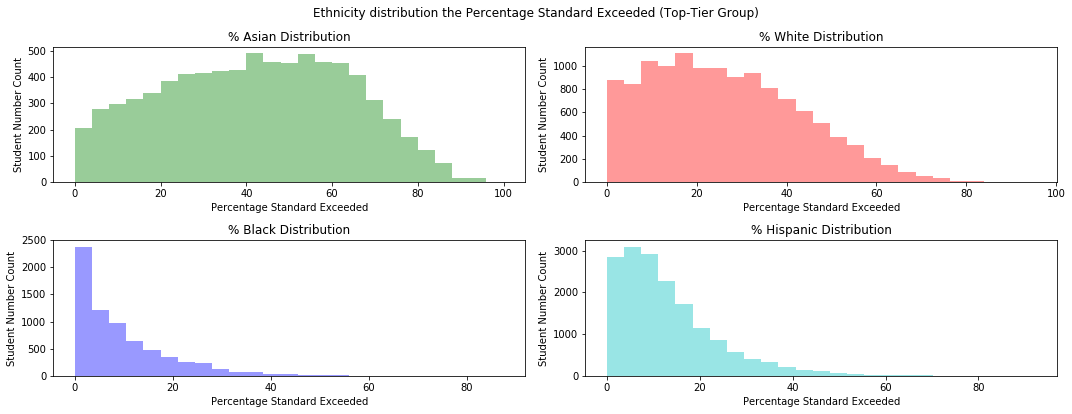
\includegraphics[width=\textwidth]{output_113_0.png}
         \caption{All achievement levels}
         \label{fig:Ethnicity_distribution_top_4}
\end{subfigure}
\hfill
\begin{subfigure}{0.45\textwidth}
         \centering
         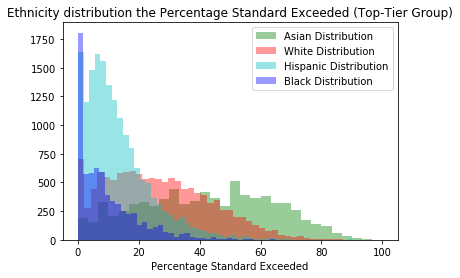
\includegraphics[width=\textwidth]{output_115_0.png}
         \caption{Comparison of highest and lowest achievement levels 
in English and Mathematics}
         \label{fig:Ethnicity_distribution_top_1}
\end{subfigure}
\hfill
\begin{subfigure}{0.45\textwidth}
         \centering
         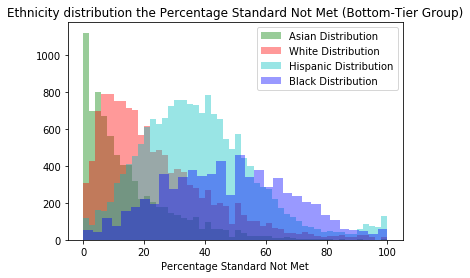
\includegraphics[width=\textwidth]{output_117_0.png}
         \caption{Comparison of highest and lowest achievement levels 
in English and Mathematics}
         \label{fig:Ethnicity_distribution_bottom_1}
\end{subfigure}
\caption{Ethnicity distribution in top and bottom scores.}
\label{fig:Ethnicity_distribution}
\end{figure}

\subsubsection{English-Language Fluency}
\textbf{Figure \ref{fig:all_English} shows that Initial Fluent English Proficient (IFEP) students achieve the best performance in both English and mathematics.}

\begin{itemize}
	\item In California, students whose home language is not English are required by law to be assessed in English language proficiency. Thus, the IFEP students have enough language proficiency or are native language speakers, and their parents may have moved from other countries and are immigrants. \textbf{This is very interesting insights that IFEP students highly exceed English only students in both English and mathematics.} The percentage of standard exceeded students of IFEP are 38.2\% (English) and 33.1\% (mathematics), while those of English only are 20.9\% (English) and 15.9\% (mathematics). I could observe that this trend becomes more obvious in the districts where many Asian immigrants live. From this result, \textbf{I can insist that immigrants have high educational interests and efforts.}  
\end{itemize}

\begin{figure}[h!]
\centering
\begin{subfigure}{0.35\textwidth}
         \centering
         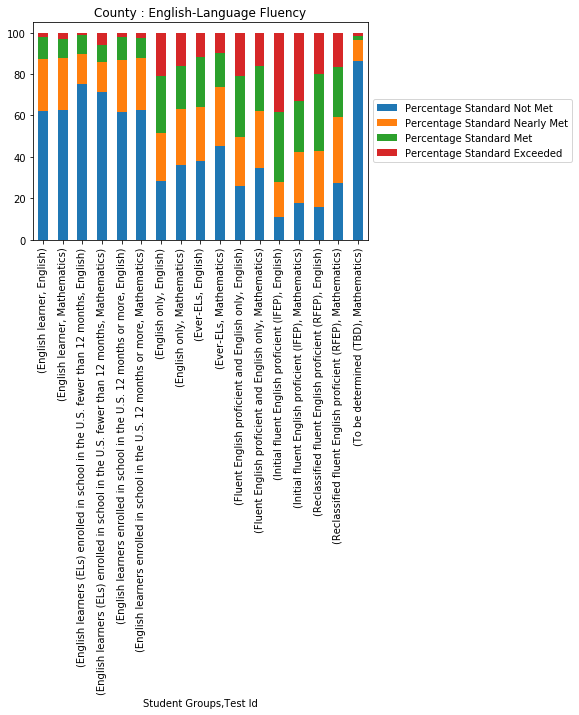
\includegraphics[width=\textwidth]{output_31_0.png}
         \caption{All achievement levels}
         \label{fig:English_all}
\end{subfigure}
\hfill
\begin{subfigure}{0.6\textwidth}
         \centering
         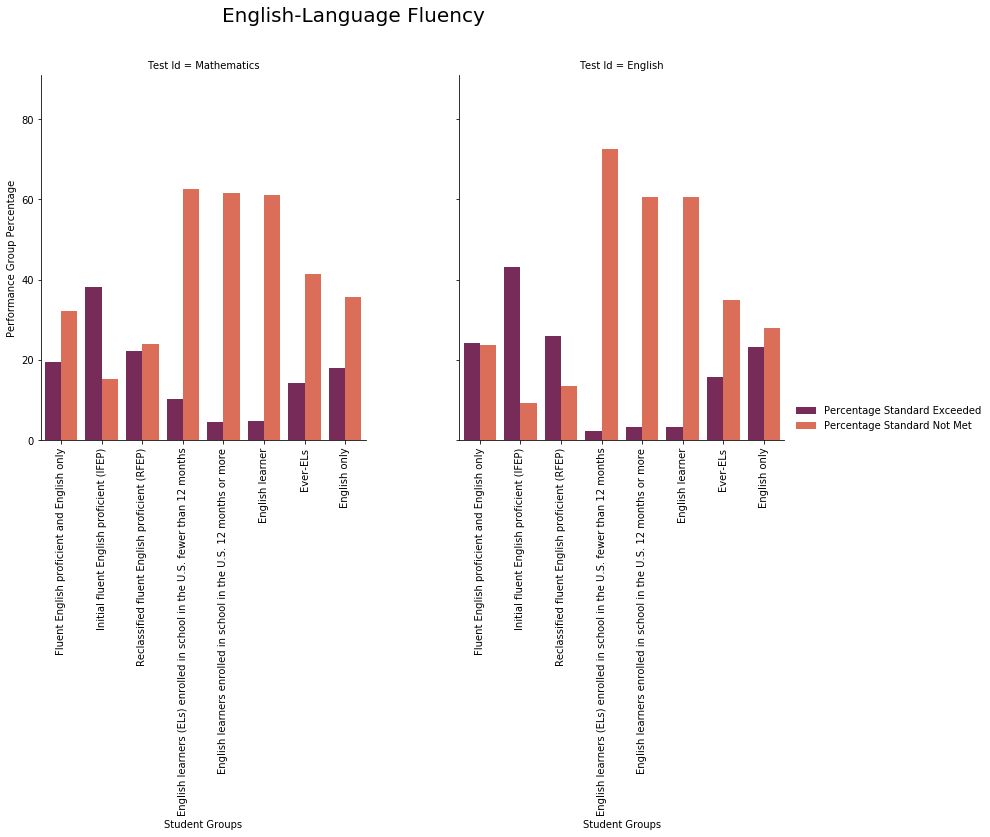
\includegraphics[width=\textwidth]{output_32_1.png}
         \caption{Comparison of highest and lowest achievement levels 
in English and Mathematics}
         \label{fig:English_two}
\end{subfigure}
\caption{Bar plots for English-Language fluency.}
\label{fig:all_English}
\end{figure}


\subsubsection{Economic Status}
\textbf{Figure \ref{fig:all_Economic} shows that the economically disadvantaged students have much more difficulties than not-economically disadvantaged students.}
\begin{itemize}
	\item \textbf{Almost half of the economically disadvantaged students are NOT standard met in mathematics.} For example, 45.4\% of economically disadvantaged students are "Standard Not Met" in mathematics and 37.4\% are "Standard Not Met" in English. 
\end{itemize}
 
\begin{figure}[h!]
\centering
\begin{subfigure}{0.35\textwidth}
         \centering
         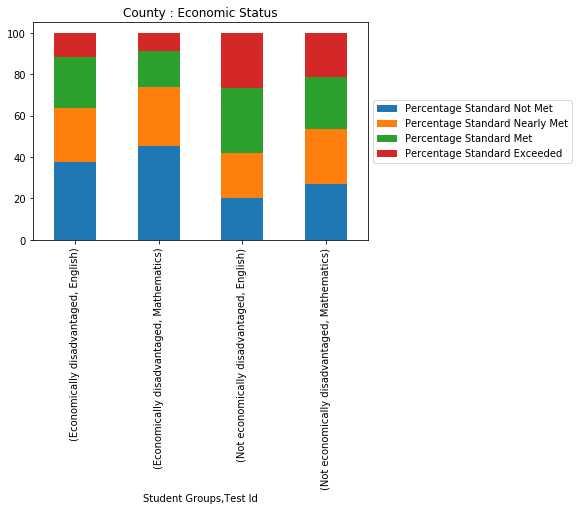
\includegraphics[width=\textwidth]{output_34_0.png}
         \caption{All achievement levels}
         \label{fig:Economic_all}
\end{subfigure}
\hfill
\begin{subfigure}{0.6\textwidth}
         \centering
         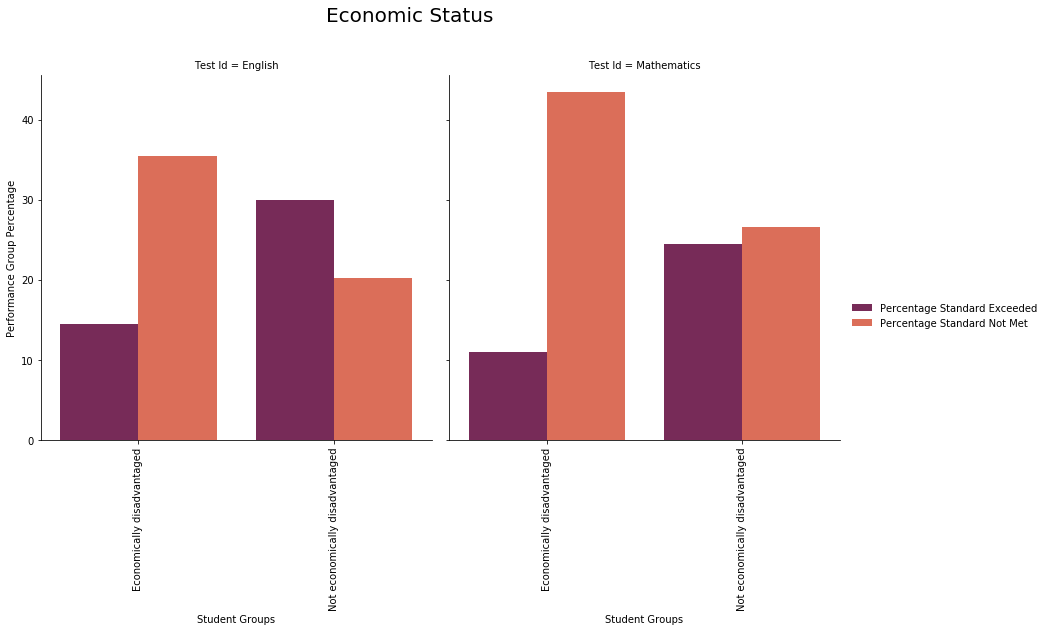
\includegraphics[width=\textwidth]{output_35_1.png}
         \caption{Comparison of highest and lowest achievement levels 
in English and Mathematics}
         \label{fig:Economic_two}
\end{subfigure}
\caption{Bar plots for economic status.}
\label{fig:all_Economic}
\end{figure}

    
 \subsubsection{Disability Status}
\textbf{Figure \ref{fig:all_Disability} shows that only the small number of students with disabilities (English: 4.6\%, mathematics: 4.5\%) could achieve the best performance}.
\begin{itemize}
	\item The majority of students with disabilities are in the "Standard Not Met" level (English: 66.7\%, mathematics: 71.1\%).
\item As in other disadvantaged or minor groups, the students with disability have more difficulties in mathematics. 
\end{itemize}

\begin{figure}[h!]
\centering
\begin{subfigure}{0.35\textwidth}
         \centering
         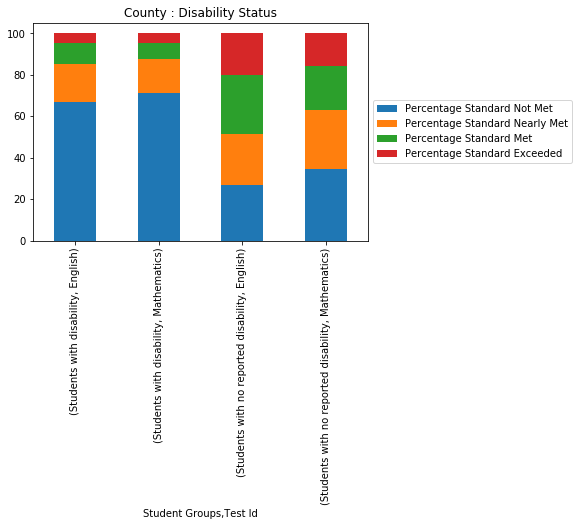
\includegraphics[width=\textwidth]{output_37_0.png}
         \caption{All achievement levels}
         \label{fig:Disability_all}
\end{subfigure}
\hfill
\begin{subfigure}{0.6\textwidth}
         \centering
         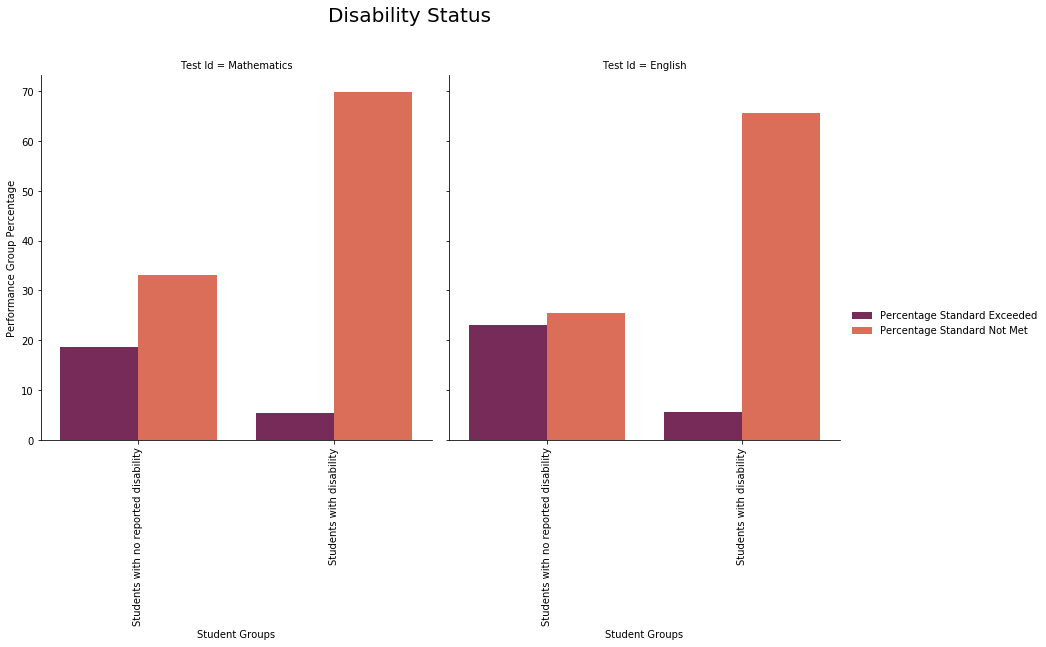
\includegraphics[width=\textwidth]{output_38_1.png}
         \caption{Comparison of highest and lowest achievement levels 
in English and Mathematics}
         \label{fig:Disability_two}
\end{subfigure}
\caption{Bar plots for disability status.}
\label{fig:all_Disability}
\end{figure}

    
\subsubsection{Parent Education}
\textbf{Figure \ref{fig:all_Education} shows that the higher the level of parental education, the higher the achievement of students.}
\begin{itemize}
	\item The graphs apparently show that \textbf{students' achievements are higher in the order of the parents' education of "graduate school/post graduate", "college graduate", "some college (includes AA degree)" , "high school graduate", and "not a high school graduate".}
\end{itemize}

\begin{figure}[h!]
\centering
\begin{subfigure}{0.35\textwidth}
         \centering
         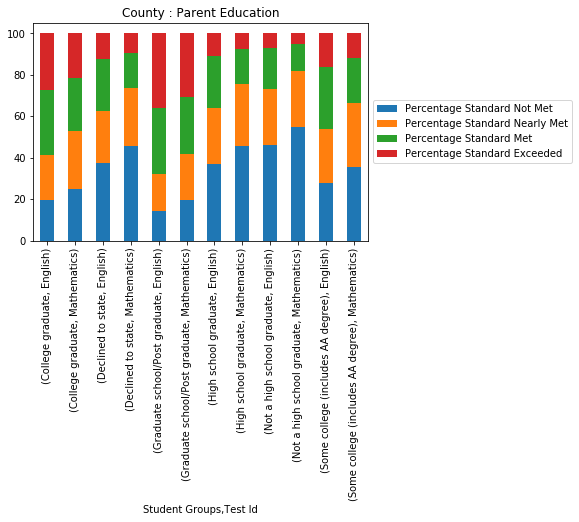
\includegraphics[width=\textwidth]{output_40_0.png}
         \caption{All achievement levels}
         \label{fig:Education_all}
\end{subfigure}
\hfill
\begin{subfigure}{0.6\textwidth}
         \centering
         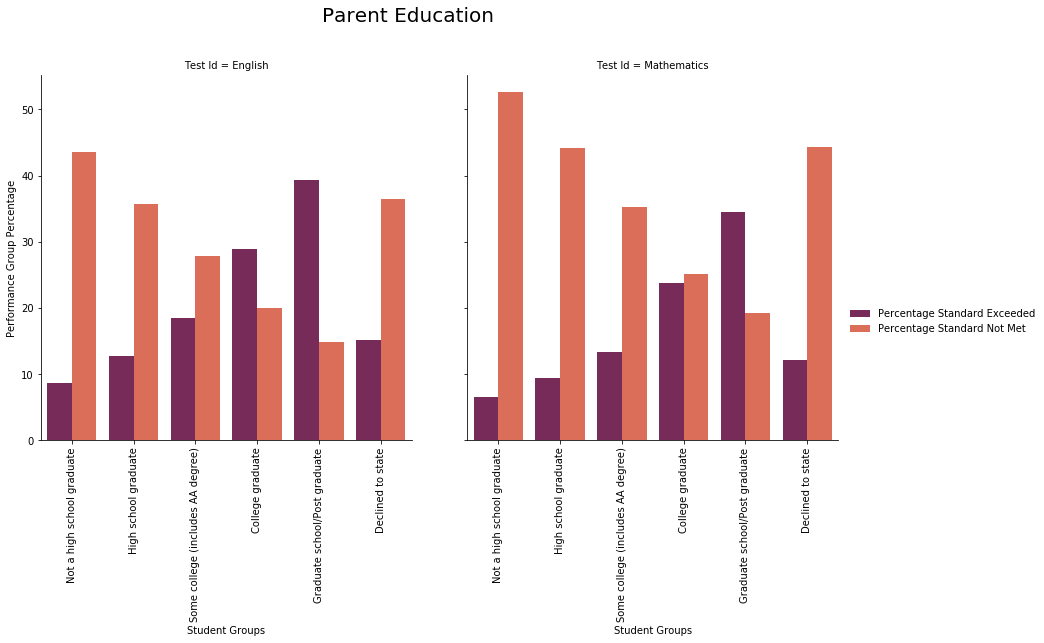
\includegraphics[width=\textwidth]{output_41_1.png}
         \caption{Comparison of highest and lowest achievement levels 
in English and Mathematics}
         \label{fig:Education_two}
\end{subfigure}
\caption{Bar plots for parent education.}
\label{fig:all_Education}
\end{figure}

%\subsection{Comparison in Best or Worst Performance Counties Using Bar Plots}

\subsection{Comparison in Best or Worst Performance Groups Using Bar Plots}
\label{Comparison for Top and Low Performance Groups Using Bar Plots}

We analyzed the best and worst 10\% performing counties (10\% out of 58 = 5 counties). The counties can be summarized as follows.
\begin{itemize}
\item Top 5 County Names in English: $[$'Santa Clara', 'Marin', 'Placer', 'San Mateo', 'Orange'$]$
\item Top 5 County Names in Mathematics: $[$'Santa Clara', 'Marin', 'San Mateo', 'Orange', 'Placer'$]$
\item Bottom 5 County Names in English: $[$'Lake', 'Kings', 'Colusa', 'Humboldt', 'Monterey'$]$
\item Bottom 5 County Names in Mathematics: $[$'Lake', 'Kings', 'Merced', 'Mendocino', 'Monterey'$]$
\end{itemize}

To have a rough insight, we have drawn the graphs of the percentage of each achievement level 
for counties (``Performance Group" ) in Figure \ref{fig:pct_each_performance_group}. 
Unfortunately, many counties have the most highest percentages in ``Percentage Standard Not Met". In addition, the differences are much bigger in two both and worst achievement levels (i.e., ``Percentage Standard Exceeded" and ``Percentage Standard Not Met") than others. Therefore, it is worth to deeply investigate those best and worst groups to find the features that can effectively help to make better performing schools.

\begin{figure}[h!]
\centering 
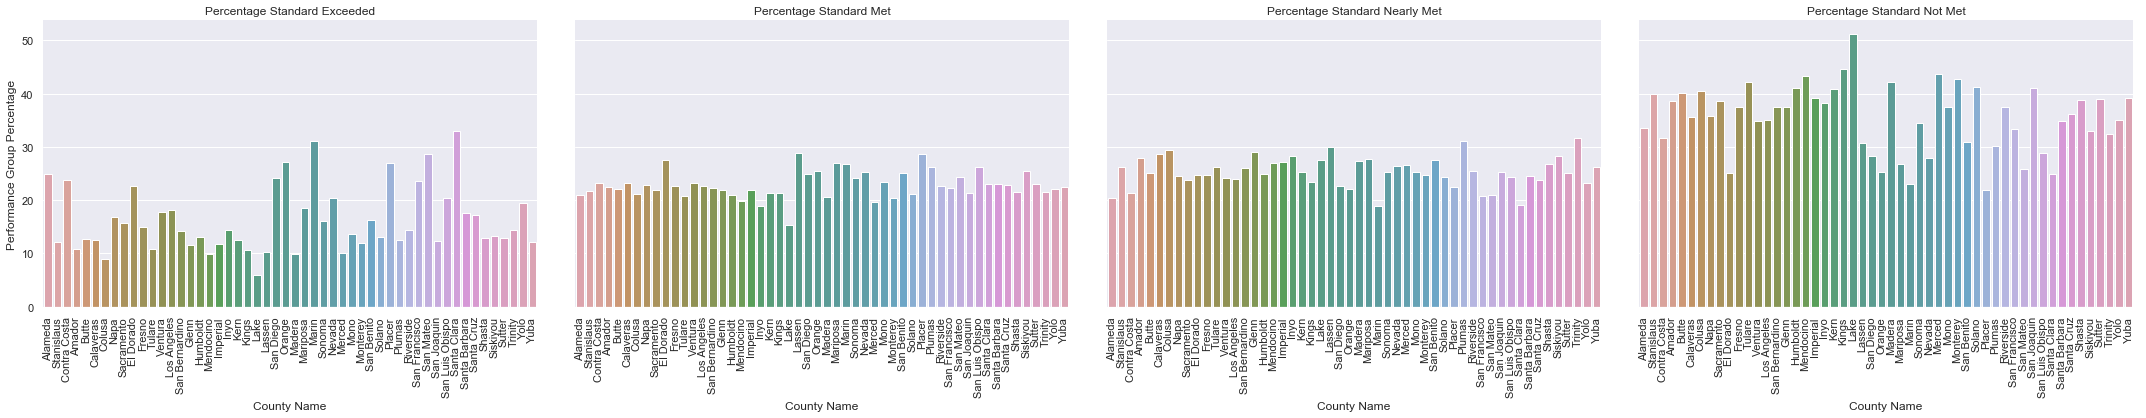
\includegraphics[width=\textwidth]{output_46_0.png}
\caption{Percentage of each achievement level for counties (``Performance Group" ).}
  \label{fig:pct_each_performance_group}
\end{figure}


\subsubsection{House Prices}

Figure \ref{fig:house_price_best_worst_counties} shows that the best performance counties have higher house median prices. In contrast, the worst performance counties have lower house median prices. Thus, \textbf{test performance is closely related to the economic capabilities of the family to which the student belongs.}

\begin{figure}[h!]
\centering
\begin{subfigure}{0.48\textwidth}
         \centering
         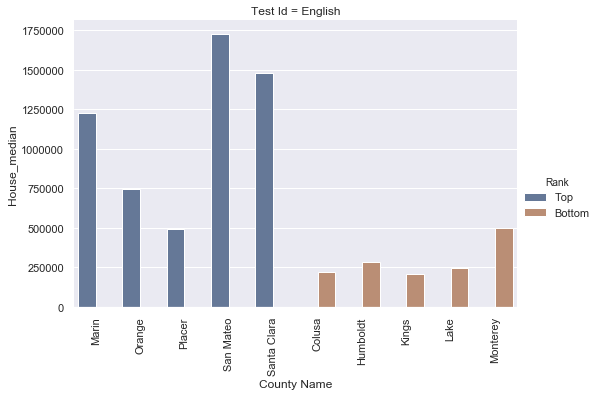
\includegraphics[width=\textwidth]{output_50_0.png}
         \caption{English}
         \label{fig:house_price_best_worst_counties_english}
\end{subfigure}
\hfill
\begin{subfigure}{0.48\textwidth}
         \centering
         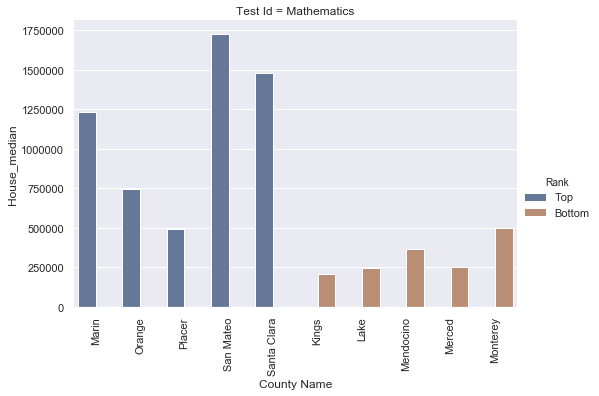
\includegraphics[width=\textwidth]{output_50_1.png}
         \caption{Mathematics}
         \label{fig:house_price_best_worst_counties_math}
\end{subfigure}
\caption{House Prices in Best and Worst 10\% Performing Counties.}
\label{fig:house_price_best_worst_counties}
\end{figure}

\subsubsection{Student Categories}

Figure \ref{fig:num_best_worst_counties} shows that the number of students in each student categories for best or worst performance groups. Here we summarize the results.

\begin{itemize}
	\item  We found that in the best performing counties, the percentage of white students is much higher than the percentage of white students in the whole county.
\item Hispanic and Latino students are far more likely to be in the worst performing group than the best performing group. Likewise, Black and American Indian students are more involved in the group with the worst results. In contrast, Asian and white students are more likely to be in the best performing group than the worst performing group.
\item The English learners have more difficulties in studying both English and Mathematics than the fluent English speakers.
\item When students' parents graduate from graduate schools/post graduates or colleges, students are much more likely to be in the best performing group. For those students, the best performing groups are much larger than the worst performing groups. In contrast, students are more likely to be in the worst performing group when their parents are high school graduates or have lower education.
\end{itemize}
 
\begin{figure}[h!]
\centering
\begin{subfigure}{0.49\textwidth}
         \centering
         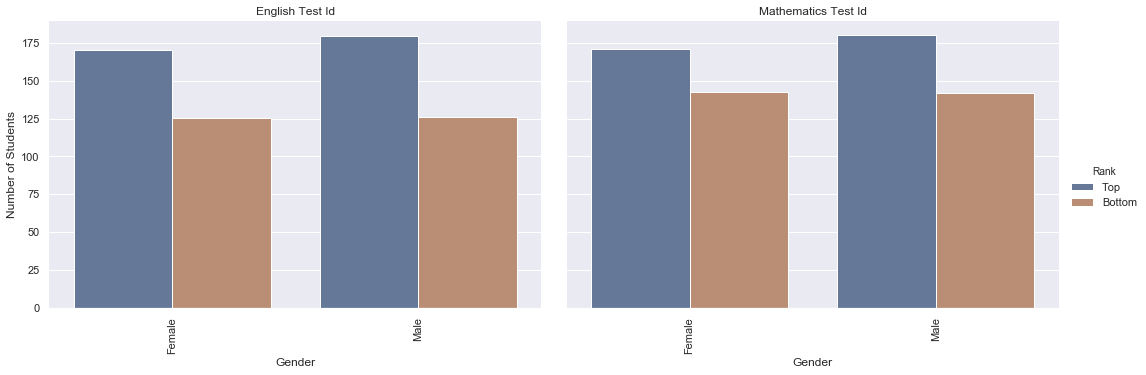
\includegraphics[width=\textwidth]{output_53_0.png}
         \caption{Gender}
         \label{fig:num_best_worst_counties_gender}
\end{subfigure}
\hfill
\begin{subfigure}{0.49\textwidth}
         \centering
         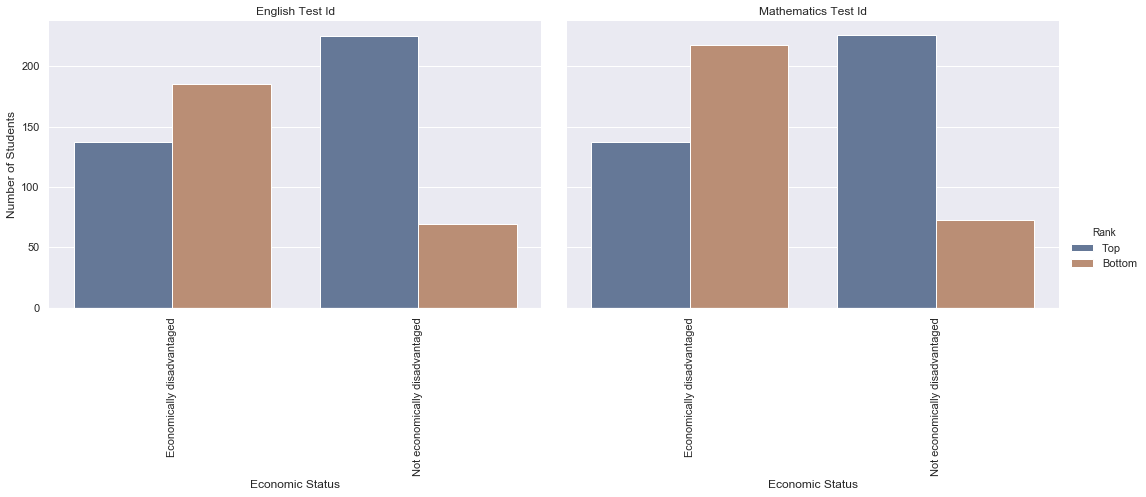
\includegraphics[width=\textwidth]{output_59_0.png}
         \caption{Economic Status}
         \label{fig:num_best_worst_counties_economic}
\end{subfigure}
\hfill
\begin{subfigure}{0.5\textwidth}
         \centering
         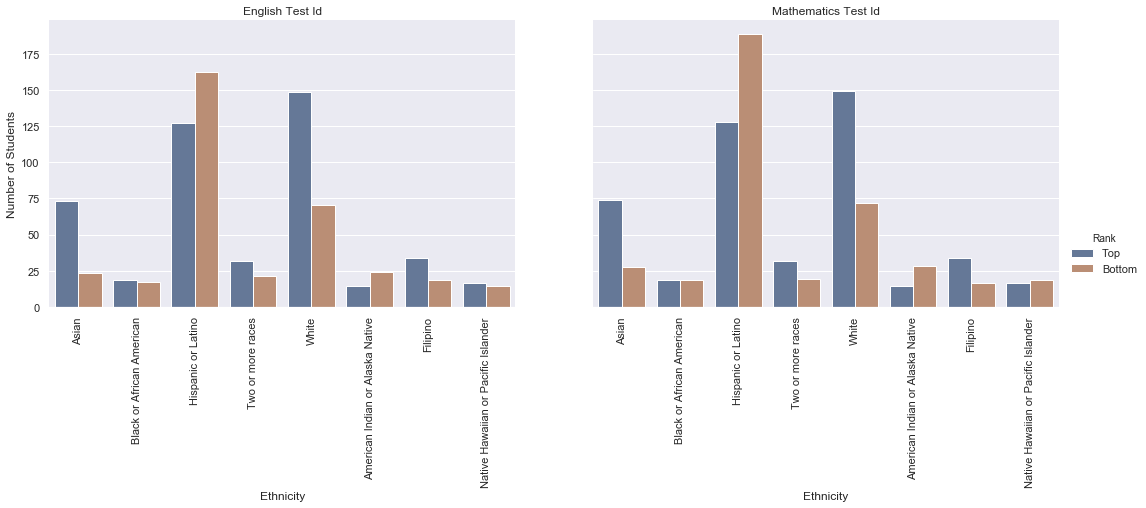
\includegraphics[width=\textwidth]{output_55_0.png}
         \caption{Ethnicity}
         \label{fig:num_best_worst_counties_ethnicity}
\end{subfigure}
\hfill
\begin{subfigure}{0.5\textwidth}
         \centering
         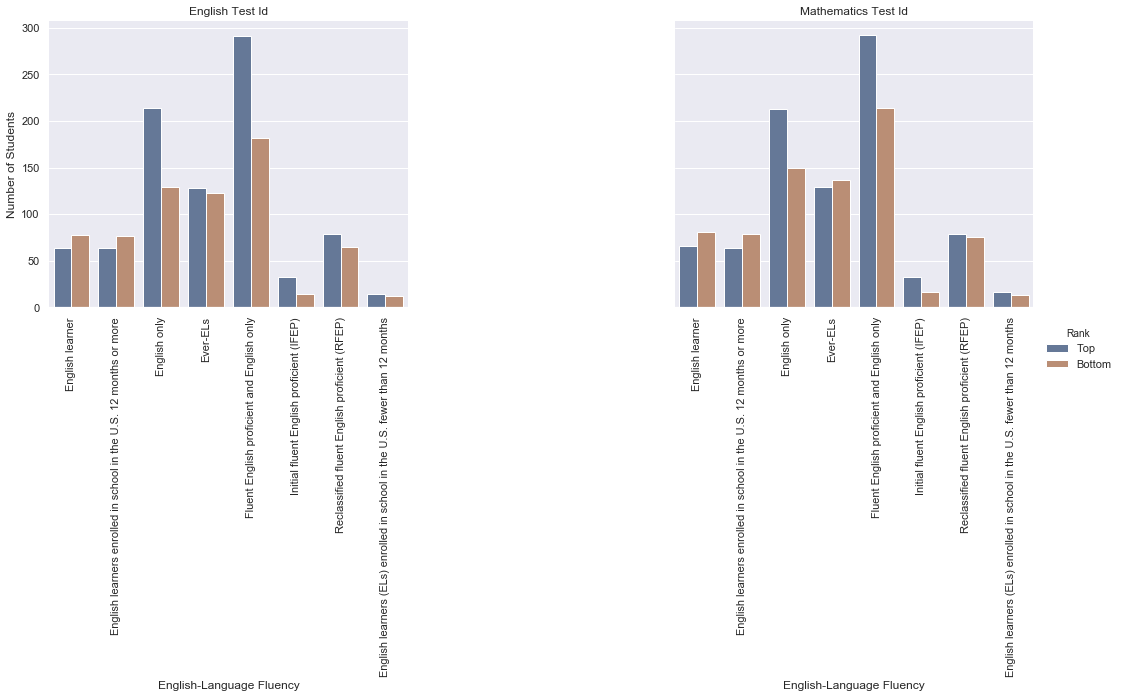
\includegraphics[width=\textwidth]{output_57_0.png}
         \caption{English-Language Fluency}
         \label{fig:num_best_worst_counties_english}
\end{subfigure}
\hfill
\begin{subfigure}{0.5\textwidth}
         \centering
         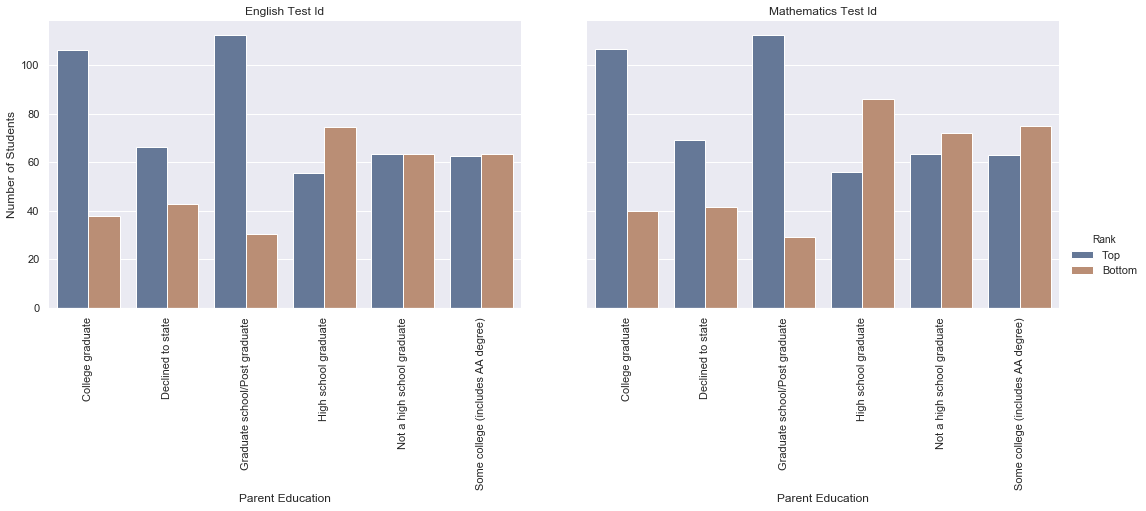
\includegraphics[width=\textwidth]{output_61_0.png}
         \caption{Parent Education}
         \label{fig:num_best_worst_counties_education}
\end{subfigure}

\caption{Number of students in each student categories for best or worst performance groups.}
\label{fig:num_best_worst_counties}
\end{figure}

\subsection{Correlations Using Scatterplots}
\label{Correlations Using Scatterplots}

\subsubsection{Test Achievements and House Prices}

As in Figure \ref{fig:house_price_vs_best}, we observe the \textbf{strong positive correlations} between the ``Percentage of Standard Exceeded" and the house prices. 
In contrast, as in Figure \ref{fig:house_price_vs_worst}, we see the \textbf{strong negative correlations} between the ``Percentage of Standard Not Met" and the house prices. 
%
In conclusion, students who live in areas with high housing prices have higher test scores.

\begin{figure}[h!]
\centering
\begin{subfigure}{0.48\textwidth}
         \centering
         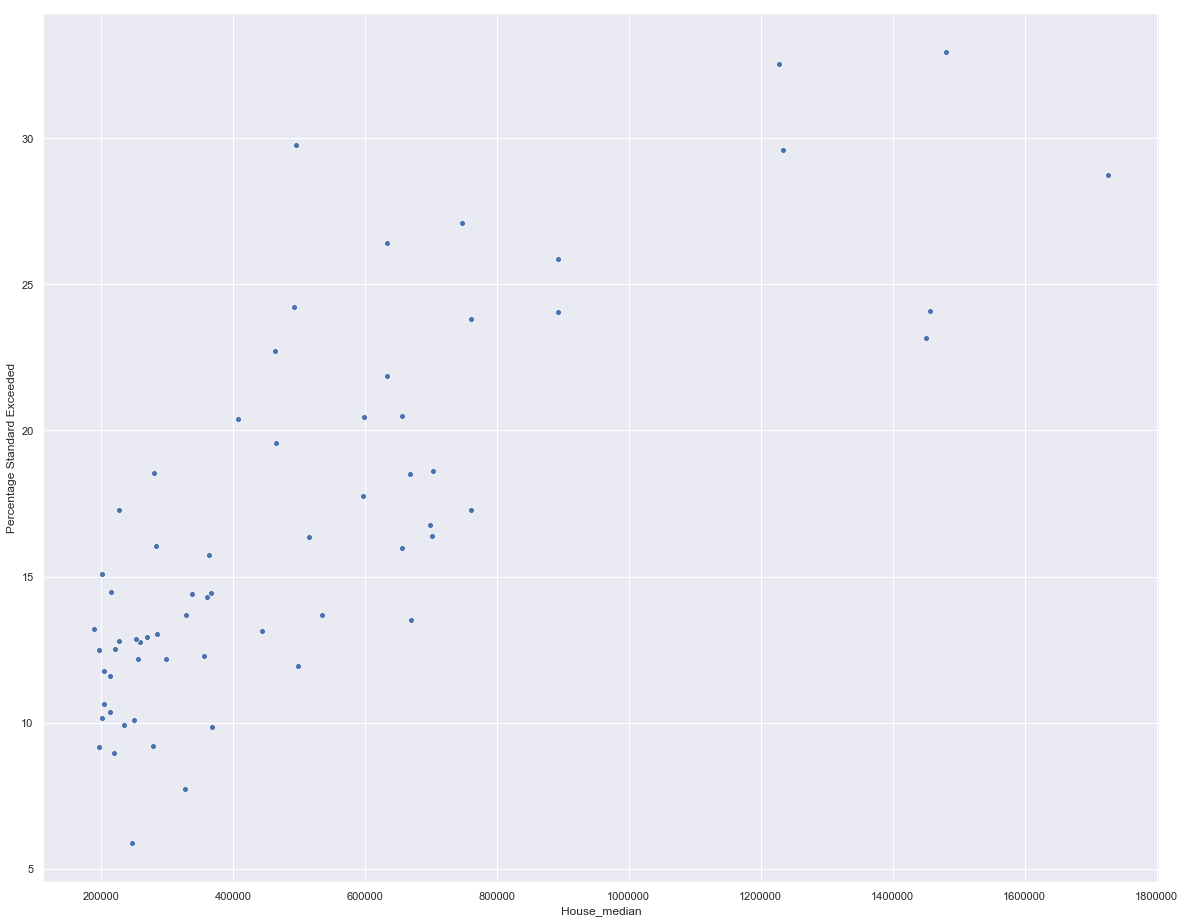
\includegraphics[width=\textwidth]{output_67_0.png}
         \caption{Percentage of Standard Exceeded vs. House Prices}
         \label{fig:house_price_vs_best}
\end{subfigure}
\hfill
\begin{subfigure}{0.48\textwidth}
         \centering
         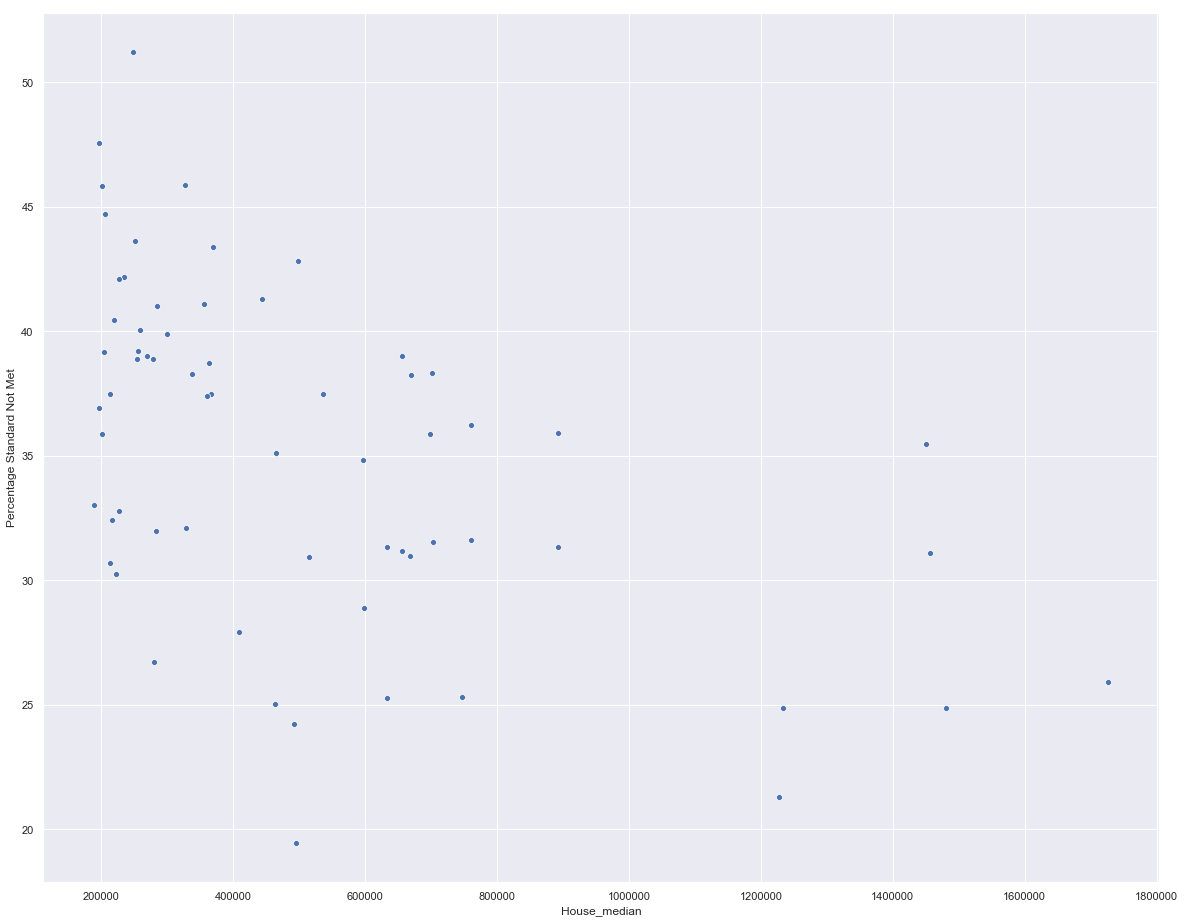
\includegraphics[width=\textwidth]{output_68_0.png}
         \caption{Percentage of Standard Not Met vs. House Prices}
         \label{fig:house_price_vs_worst}
\end{subfigure}
\caption{Correlation graphs between test scores and house prices.}
\label{fig:house_price_score_performance}
\end{figure}

\section{Exploratory Data Analysis}
\label{Exploratory Data Analysis}

In this section, we use the inferential statistics to identify significant features in the data set.
%
More details with codes on exploratory data analysis can be found in
\href{https://github.com/ahrimhan/data-science-project/blob/master/project1/exploratory_data_analysis.ipynb}{this IPython notebook}. 


Before performing exploratory data analysis, we need to preprocess the data.
%
\textbf{Each school has 47 scores for each student category group}. Each student category group is summarized in Table \ref{table:student_group}. 
%
For predicting school scores, we need to focus on the school-level instances.
%
Therefore, \textbf{we transform data for each school}.
%%
By using the \texttt{`pivot\_table'} method in Pandas,
\textbf{we need to pivot the scores based on a school as an index}.
%
Therefore, 47 scores of each student group is added as features for each school instance.


\begin{table}[h!]
\footnotesize
\centering
%\begin{tabular}{||p{0.6cm}|p{6cm}|c||}
\begin{tabular}{||c|c|c||}
  \hline
Num & Category & Student Groups\\
\hline
1 & All Students & All Students \\
\hline
2 &	\multirow{2}{*}{Gender} & Male\\ \cline{1-1}\cline{3-3}
3 &	& Female\\
\hline
4 & \multirow{8}{*}{Ethnicity} & American Indian or Alaska Native\\\cline{1-1}\cline{3-3}
5 && Asian\\\cline{1-1}\cline{3-3}
6 && Black or African American\\\cline{1-1}\cline{3-3}
7 && Filipino\\\cline{1-1}\cline{3-3}
8 && Hispanic or Latino\\\cline{1-1}\cline{3-3}
9 && Native Hawaiian or Pacific Islander\\\cline{1-1}\cline{3-3}
10 && Two or more races\\\cline{1-1}\cline{3-3}
11 && White\\
\hline
12 & \multirow{9}{*}{English-Language Fluency} & English learner (EL)\\\cline{1-1}\cline{3-3}
13 &&  ELs enrolled in school in the U.S. fewer than 12 months\\\cline{1-1}\cline{3-3}
14 && ELs enrolled in school in the U.S. 12 months or more\\\cline{1-1}\cline{3-3}
15 && English only\\\cline{1-1}\cline{3-3}
16 && Ever-ELs\\\cline{1-1}\cline{3-3}
17 && Fluent English proficient and English only\\\cline{1-1}\cline{3-3}
18 && Initial fluent English proficient (IFEP)\\\cline{1-1}\cline{3-3}
19 && Reclassified fluent English proficient (RFEP)\\\cline{1-1}\cline{3-3}
20 && To be determined (TBD)\\
\hline
21 & \multirow{6}{*}{Parent Education} & College graduate\\\cline{1-1}\cline{3-3}
22 && Declined to state\\\cline{1-1}\cline{3-3}
23 && Graduate school/Post graduate\\\cline{1-1}\cline{3-3}
24 && High school graduate\\\cline{1-1}\cline{3-3}
25 && Not a high school graduate\\ \cline{1-1}\cline{3-3}
26 && Some college (includes AA degree)\\
\hline
27 & \multirow{2}{*}{Economic Status} & Economically disadvantaged\\\cline{1-1}\cline{3-3}
28 && Not economically disadvantaged\\
\hline
29 & \multirow{2}{*}{Disability Status} & Students with disability\\\cline{1-1}\cline{3-3}
30 && Students with no reported disability\\
\hline
31 & Migrant & Migrant education\\
\hline
32 & \multirow{8}{*}{Ethnicity for Economically Disadvantaged} & American Indian or Alaska Native\\\cline{1-1}\cline{3-3}
33 && Asian\\\cline{1-1}\cline{3-3}
34 && Black or African American\\\cline{1-1}\cline{3-3}
35 && Filipino\\\cline{1-1}\cline{3-3}
36 && Hispanic or Latino\\\cline{1-1}\cline{3-3}
37 && Native Hawaiian or Pacific Islander\\\cline{1-1}\cline{3-3}
38 && Two or more races\\\cline{1-1}\cline{3-3}
39 && White\\
\hline
40 & \multirow{8}{*}{Ethnicity for Economically Not Disadvantaged} & American Indian or Alaska Native\\\cline{1-1}\cline{3-3}
41 && Asian\\\cline{1-1}\cline{3-3}
42 && Black or African American\\\cline{1-1}\cline{3-3}
43 && Filipino\\\cline{1-1}\cline{3-3}
44 && Hispanic or Latino\\\cline{1-1}\cline{3-3}
45 && Native Hawaiian or Pacific Islander\\\cline{1-1}\cline{3-3}
46 && Two or more races\\\cline{1-1}\cline{3-3}
47 && White\\
\hline
\end{tabular}
\caption{47 student category groups.}
\label{table:student_group}
\end{table}



%For reference purpose, we provide each student category group can be summarize in the form of 'Category' = ['Student Groups'] as follows.
%\begin{itemize}
%	\item "All Students" = [All Students]
%\item "Gender" = [Male, Female]
%\item "Ethnicity" = [American Indian or Alaska Native, Asian, Black or African American, Filipino, Hispanic or Latino, Native Hawaiian or Pacific Islander, Two or more races, White]
%"English-Language Fluency" = [English learner, English learners (ELs) enrolled in school in the U.S. fewer than 12 months, English learners enrolled in school in the U.S. 12 months or more, English only, Ever-ELs, Fluent English proficient and English only, Initial fluent English proficient (IFEP), Reclassified fluent English proficient (RFEP), To be determined (TBD)]
%\item "Parent Education" = [College graduate, Declined to state, Graduate school/Post graduate, High school graduate, Not a high school graduate, Some college (includes AA degree)]
%"Migrant" = [Migrant education]
%\item
%"Economic Status" = [Economically disadvantaged, Not economically disadvantaged]
%\item
%"Disability Status" = [Students with disability, Students with no reported disability]
%\item
%"Ethnicity for Economically Disadvantaged" = [American Indian or Alaska Native, Asian, Black or African American, Filipino, Hispanic or Latino, Native Hawaiian or Pacific Islander, Two or more races, White]
%\item
%Ethnicity for Not Economically Disadvantaged = [American Indian or Alaska Native, Asian, Black or African American, Filipino, Hispanic or Latino, Native Hawaiian or Pacific Islander, Two or more races, White]
%\end{itemize}

%
We need to derive new variables (e.g., number to percentage of Asian students) and merge variables (e.g., minor groups of ethnicity such ``Native Hawaiian or Pacific Islander" and ``American Indian or Alaska Native"). More detailed explanation for variables is in Section \ref{Variables for Modeling}.

\textbf{A significant number of features could be redundant and irrelevant, therefore it is important to apply feature selection/dimension reduction}.
%
We performed the statistical hypothesis testing, correlation test, and feature selection for
getting rid of the student group information for generating less number of features. In other words, we aim to generate and use the features that strongly affect for predicting the school scores.

%Having all features either would not help building a real predictive model
% or the computation when dimensions are significantly large.
%
%Therefore, it is important to identify the essential features for predicting a target variable.

\subsection{Statistical Hypothesis Testing}

\subsubsection{T-Test for means of two independent samples.}

We test whether the means of two independent samples are significantly different. If there is no difference (p-value is greater or equal than $\alpha$ = 0.05), then we want to \textbf{eliminate or merge} that student group information due to too much generating features.
\begin{itemize}
\item[-] $H_{0}$: There is \textbf{no difference} in students' scores between sample1 and sample2.
\item[-] $H_{1}$: There \textbf{exist difference} in students' scores between sample1 and sample2.
\end{itemize}

\paragraph*{T-Test for All Pairs.}
We performed a hypothesis test (two-sample test) for all pairs of student groups by assuming two group of samples are independent.  

Figure \ref{fig:t-test_all} shows the results that
the student group features sorted on the order of the occurrences. The following shows the results with the counter number. 
\begin{figure}[h!]
\centering 
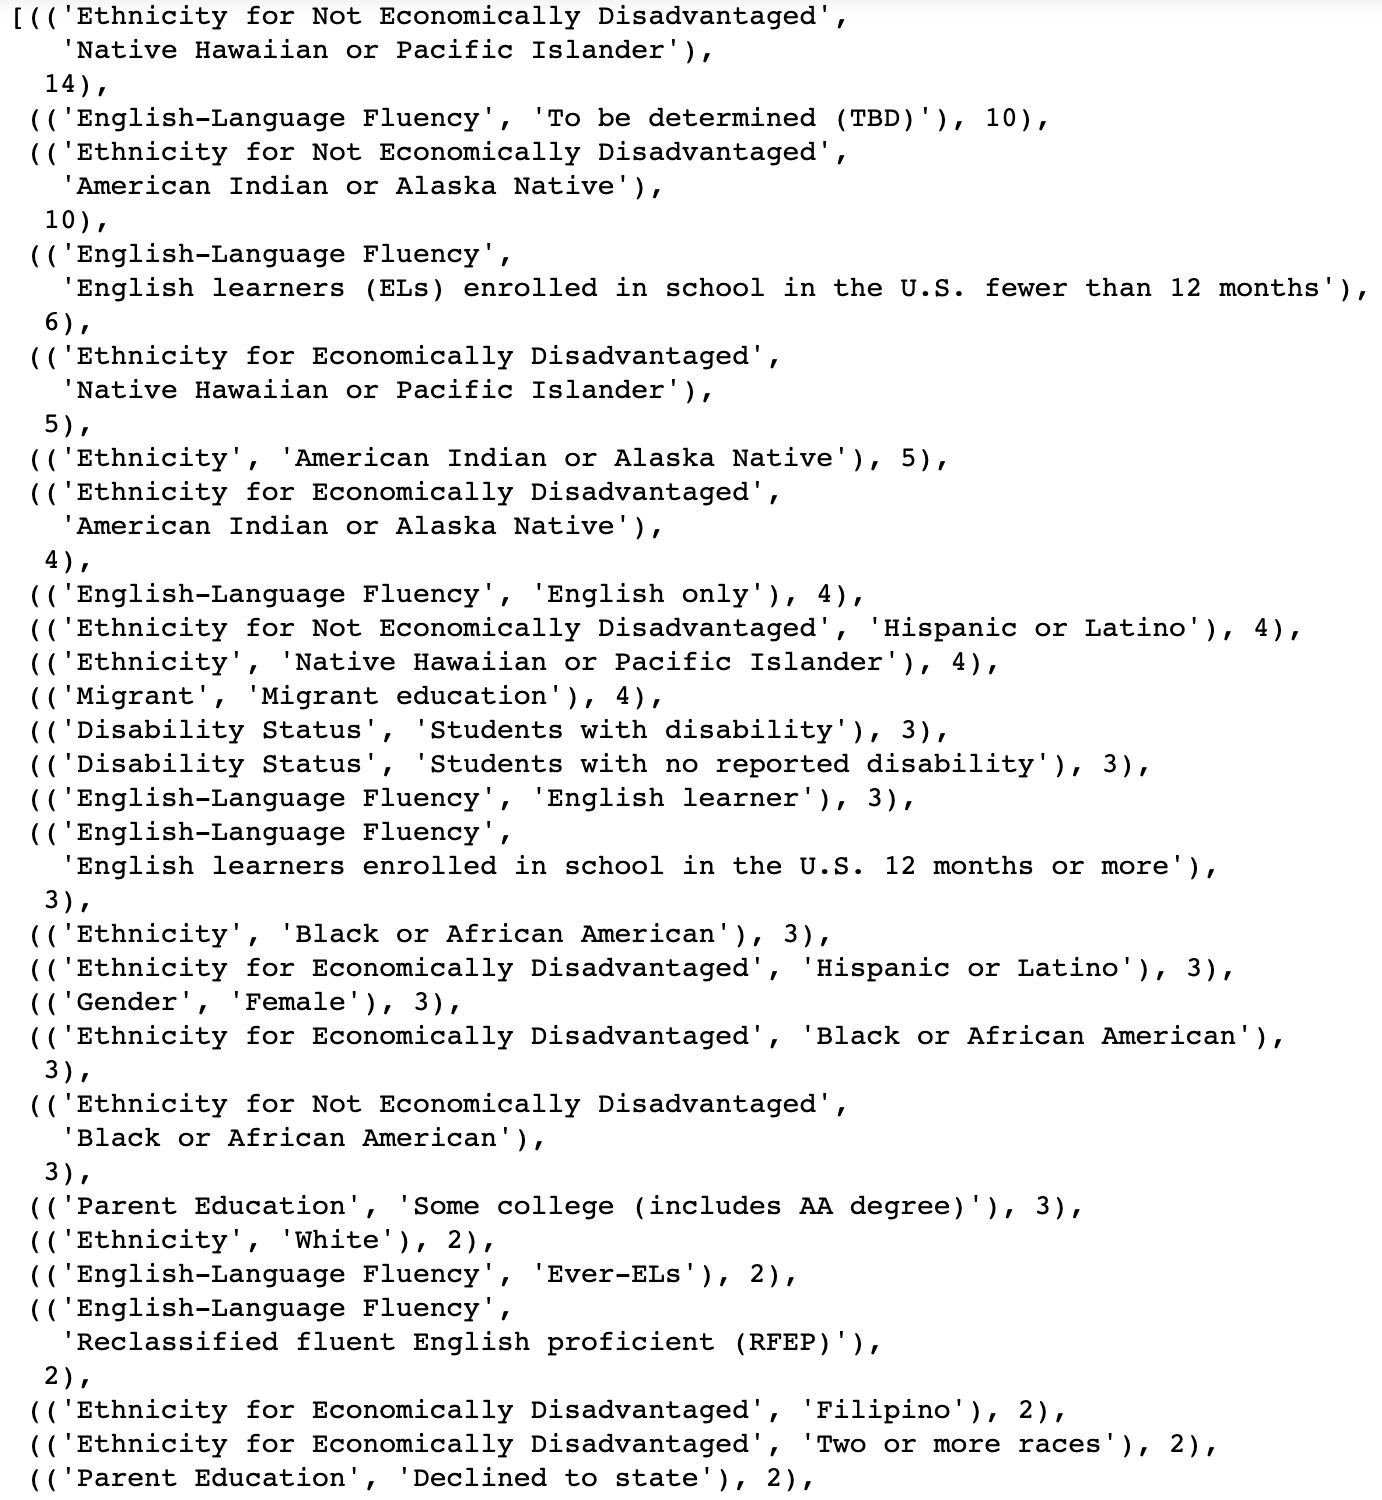
\includegraphics[width=\textwidth]{t-test_all.png}
\caption{T-test for the means of two samples for on target value 'Percentage Standard Exceeded'.}
  \label{fig:t-test_all}
\end{figure}

\paragraph*{T-Test Between English and Mathematics Subjects.}

The score differences exist in most of the groups. 
%
In these test (Figure \ref{fig:t-test_subjects}), when the  $p-$value is much smaller than $\alpha$  = 0.05, and we reject the null hypothesis that there is no difference. In fact, the $p-$values zero indicates that there is significant differences between two samples in scores. 
%
However, we eliminate the subjects (Test Id) for further analysis or constructing prediction models, because the subject difference is not our major concerns.

\begin{figure}[h!]
\centering 
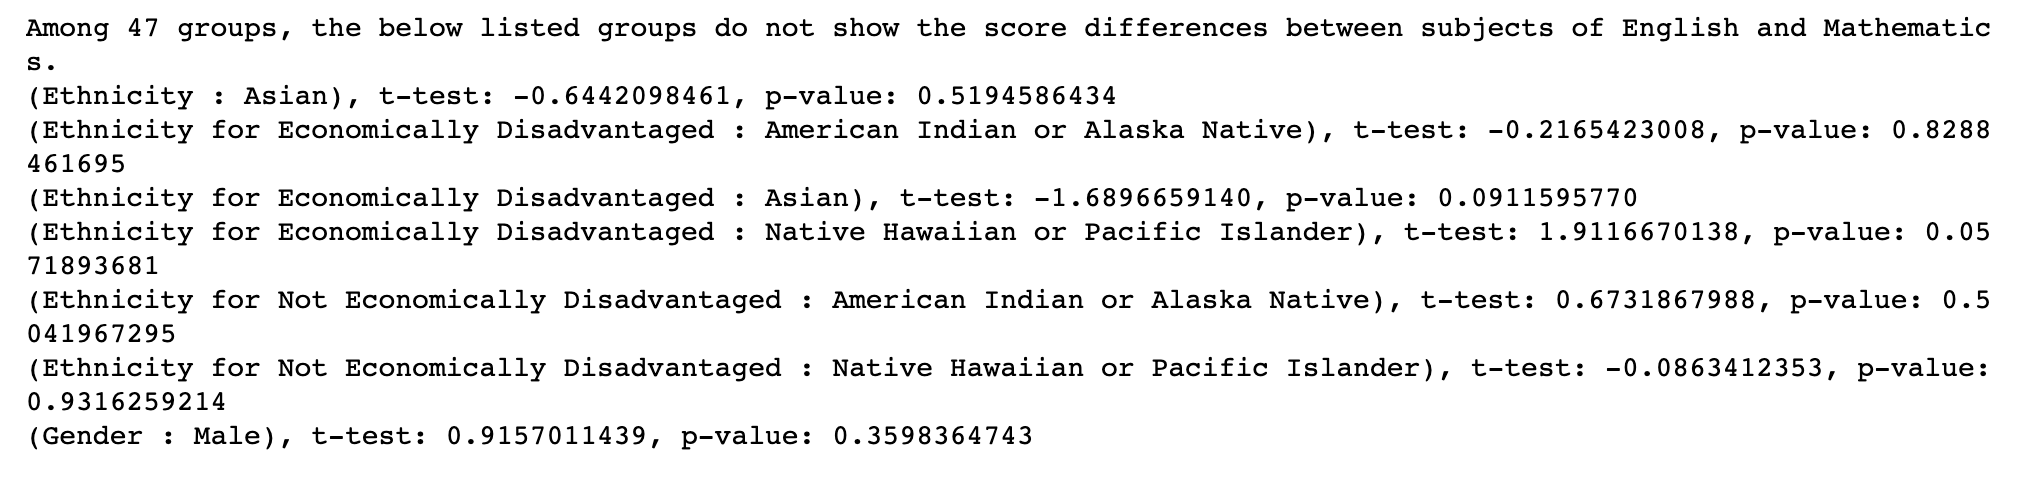
\includegraphics[width=\textwidth]{t-test_subjects.png}
\caption{T-test between subjects (English and Mathematics).}
  \label{fig:t-test_subjects}
\end{figure}

\paragraph*{Stepwise way of Feature Deletion.}
We can choose to drop all the rows of ('Category', 'Student Group') that do not actually affect a target variable, 'Percentage Standard Exceeded' or 'Percentage Standard Not Met' using the \textbf{stepwise way} for removing the student group information.

We analyzed all pairs of two samples using T-test and found the two samples that have no difference (p-value is greater or equal than $\alpha$ = 0.05). Then, we select and delete the most occurrence feature in the T-test results. 
%
We then reiterate the T-test process for find and delete next least affecting feature. The following results shows the deleted features (i.e., student group information) for every step with the number of occurrences.

\begin{figure}[h!]
\centering 
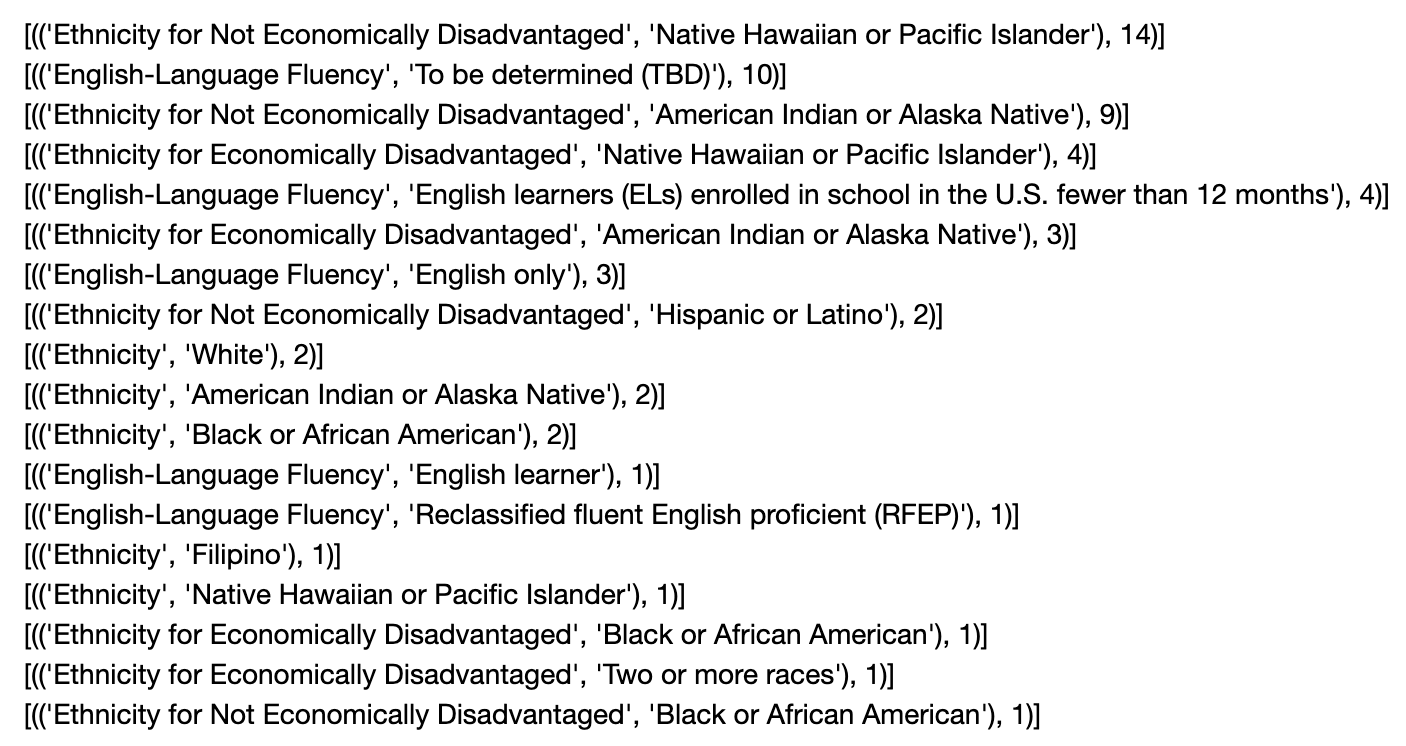
\includegraphics[width=\textwidth]{t-test_stepwise.png}
\caption{Stepwise way of feature deletion: For each iteration, we remove the feature that most occurring in the T-test results of no differences.}
  \label{fig:t-test_stepwise}
\end{figure}

\paragraph*{Decisions for Variables.}
Based on the T-test, we can eliminate or merge the weak affecting student group indicators. 
By referring the indicators determined to have no difference features, we adjust the following indicators for variables that will be used to make a machine-learning based school score prediction model.

\begin{enumerate}
	\item Delete the meaningless indicators such as, 'To be determined (TBD)' and 'Declined to state'.
\item Delete the 'Disability Status', 'Economic Status', and 'Ethnicity for Not Economically Disadvantaged'. It seems redundant and rather trivial that do not produce the new results.
\item For 'Ethnicity', delete 'Two or more races', and merge "Native Hawaiian or Pacific Islander" and "American Indian or Alaska Native" and create Minor races (i.e., Pct\_Avg\_Multi\_Ethnicity\_Minor, Pct\_Multi\_Ethnicity\_Minor\_English, and Pct\_Multi\_Ethnicity\_Minor\_Mathematics).
\item For 'English-Language Fluency', we organize the indicators:
\begin{itemize}
	\item Delete 'English learners (ELs) enrolled in school in the U.S. fewer than 12 months' and 'English learners enrolled in school in the U.S. 12 months or more' and use the 'English learner' only instead
\item Delete 'Ever-ELs' which indicates 'Reclassified fluent English proficient (RFEP)' + 'English learner'
\end{itemize}  
\item For 'Parent Education', delete 'Some college (includes AA degree)'
\end{enumerate}

\subsection{Correlation Tests}

Correlation represents how the features are related to each other or to the target variable.
%
Correlation can be positive (increase in one value of feature increases the value of the target variable) or negative (increase in one value of feature decreases the value of the target variable).

\subsubsection{Matrix with Heatmap}

Heatmap makes it easy to identify which features are most related to the target variable, we will plot heatmap of correlated features using the seaborn library.

\paragraph*{Correlation Table with Number/Percentage Related Features.}

\begin{figure}[h!]
\centering 
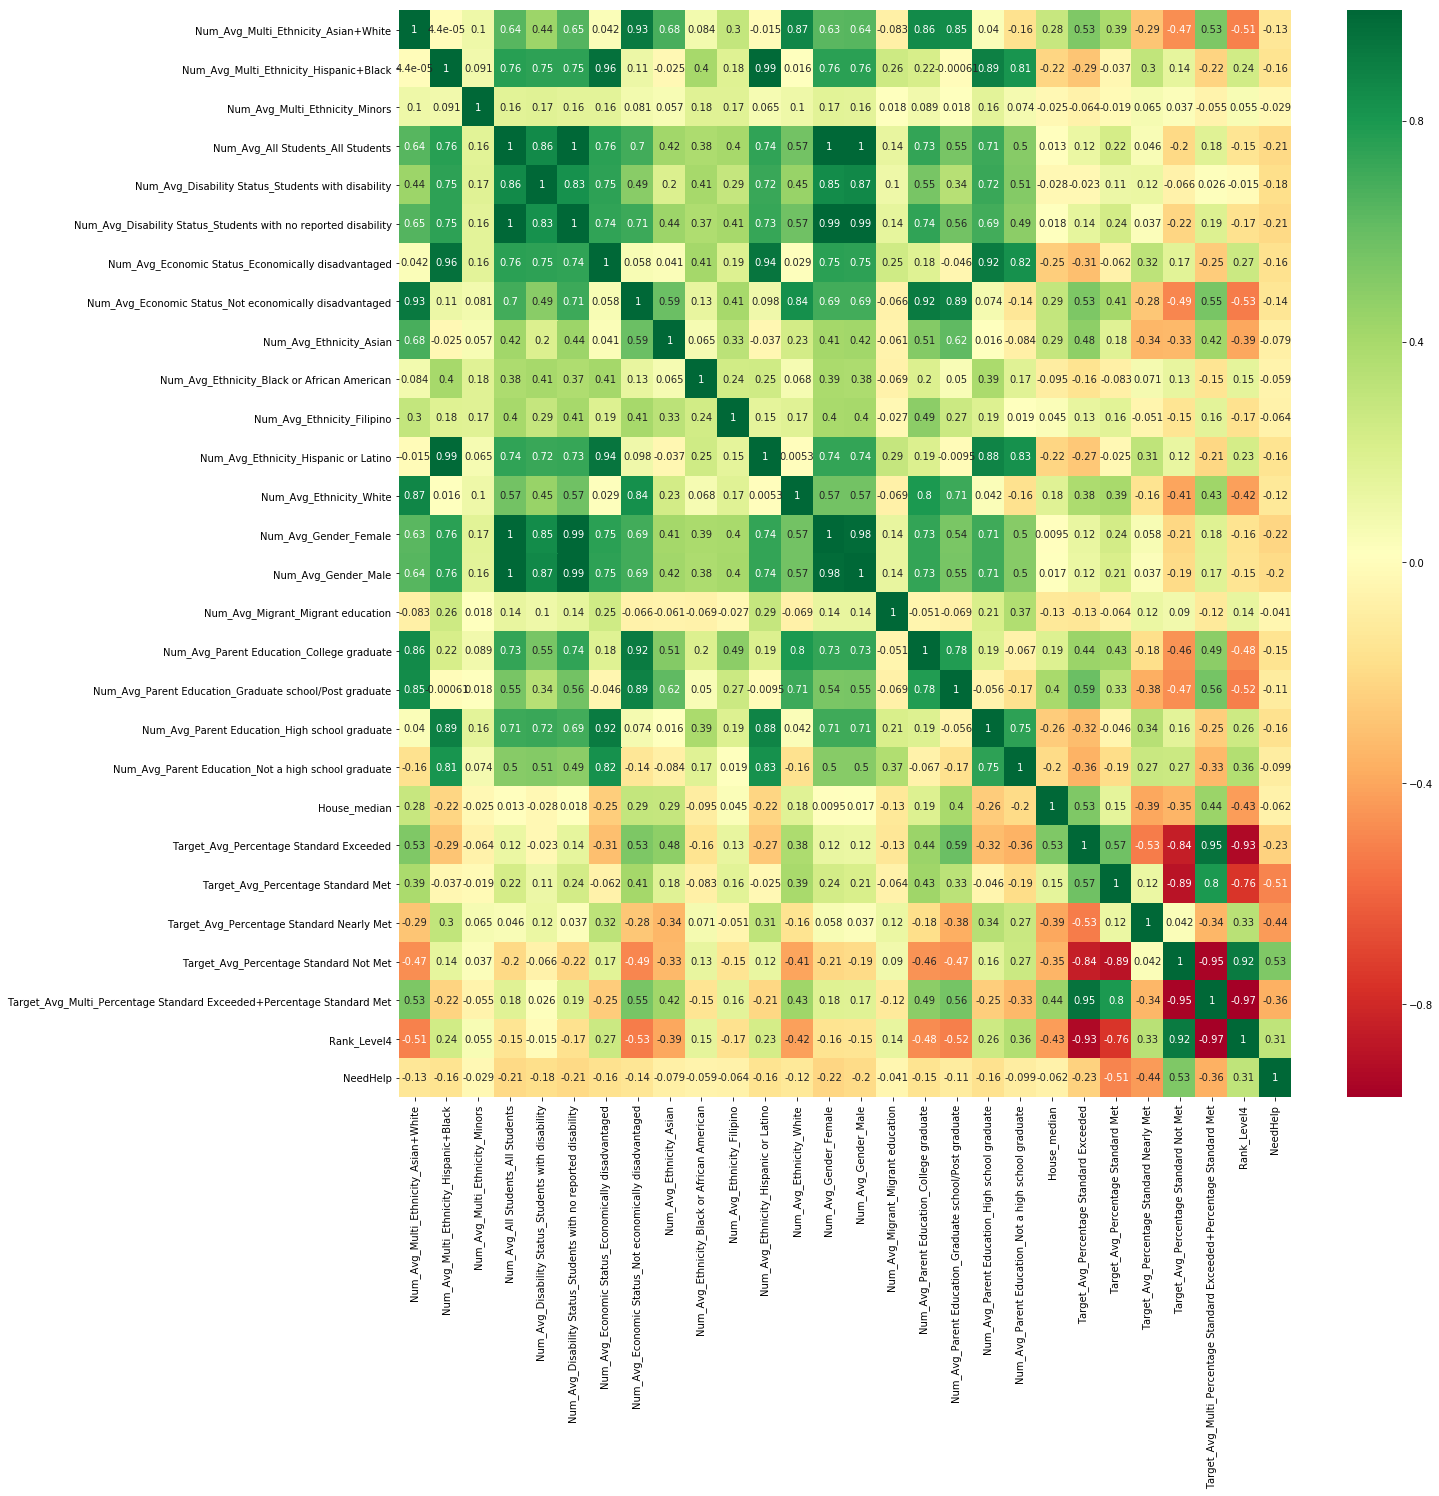
\includegraphics[width=\textwidth]{output_83_0.png}
\caption{Correlation Table with Number Related Features.}
  \label{fig:corr_num}
\end{figure}

\begin{figure}[h!]
\centering 
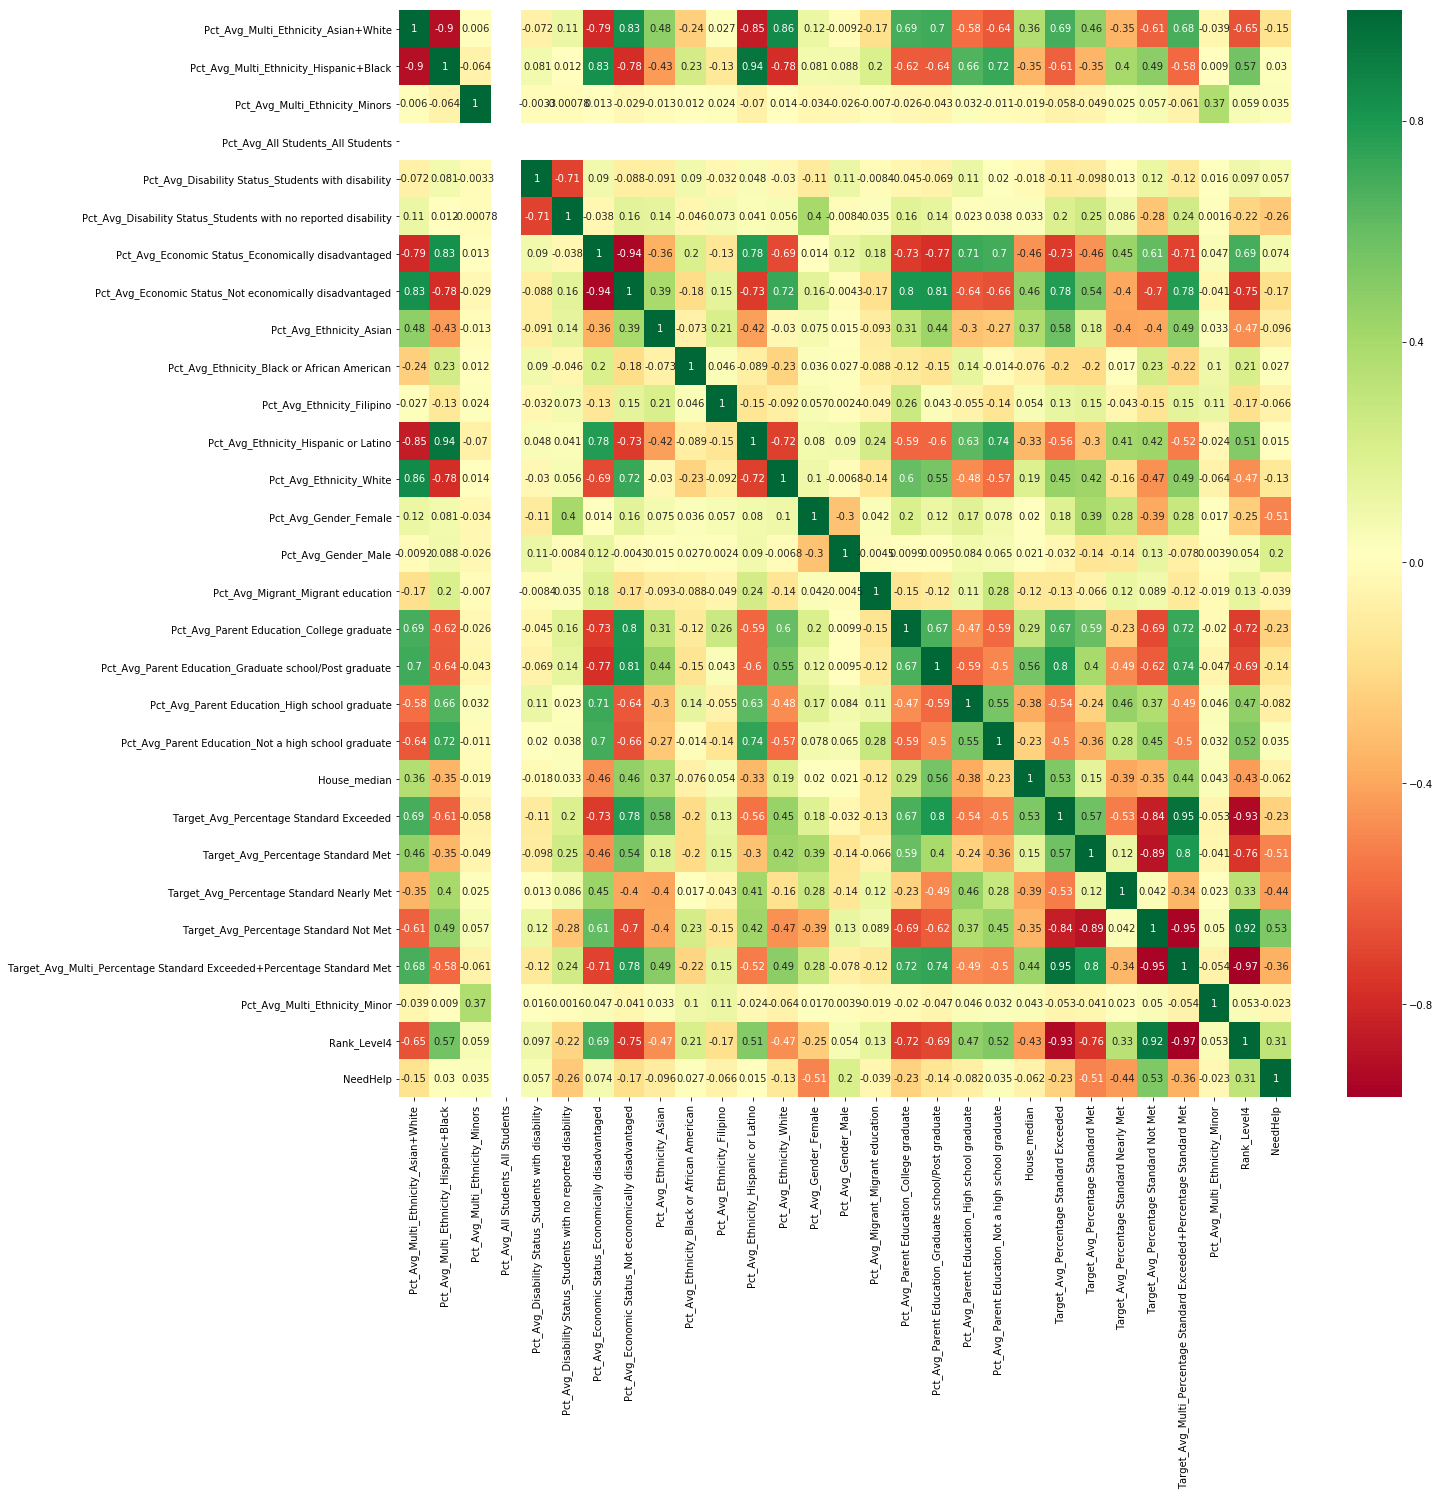
\includegraphics[width=\textwidth]{output_85_0.png}
\caption{Correlation Table with Percentage Related Features.}
  \label{fig:corr_pct}
\end{figure}

Figure \ref{fig:corr_num} and Figure \ref{fig:corr_pct} show that, just as assumed, the high score (`Target\_Avg\_Percentage Standard Exceeded`) is correlated to the higher house price (`House\_median`), the higher education (`Num\_Avg\_Parent Education\_Graduate school/Post graduate`), and good economic status (`Num\_Avg\_Economic Status\_Not economically disadvantaged`).  

It is interesting that the number of Hispanics (`Num\_Avg\_Ethinicity\_Hispanic or Latino`) is highly correlated (\textbf{0.94}) with the number of economically disadvantaged students. The percent of Hispanics (`Pct\_Avg\_Ethinicity\_Hispanic or Latino`) is correlated (\textbf{0.78}) but not as strong as the number feature.
In California, there is the largest number of Hispanic students compared to other ethnicity students (see Figure \ref{fig:num_ethnicity}), and this can be the cause of the high correlation.

\begin{figure}[h!]
\centering 
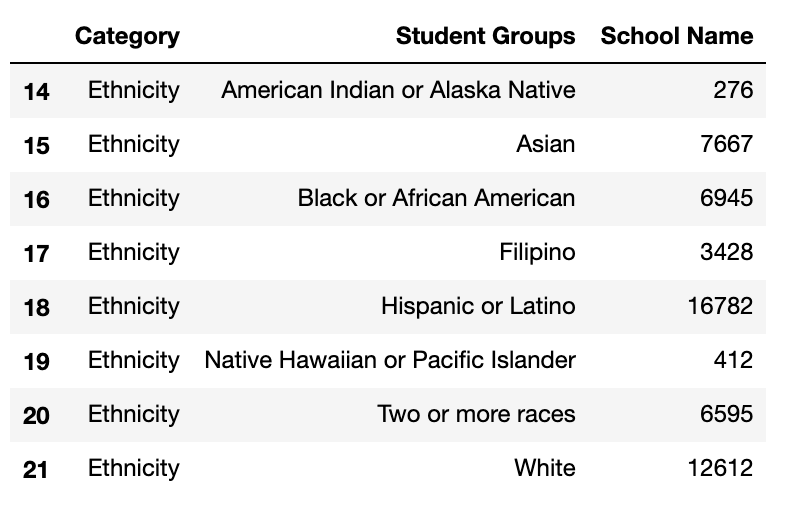
\includegraphics[scale=0.8]{num_ethnicity.png}
\caption{Number of collected school data for each ethnicity.}
  \label{fig:num_ethnicity}
\end{figure}

%\paragraph*{Correlation Table in Specific Inferior Group.}
%
%We specifically obtained the Heatmap correlation table for this inferior group. The results are represented in Figure \ref{fig:corr_inferior}.
%
%\begin{figure}[h!]
%\centering 
%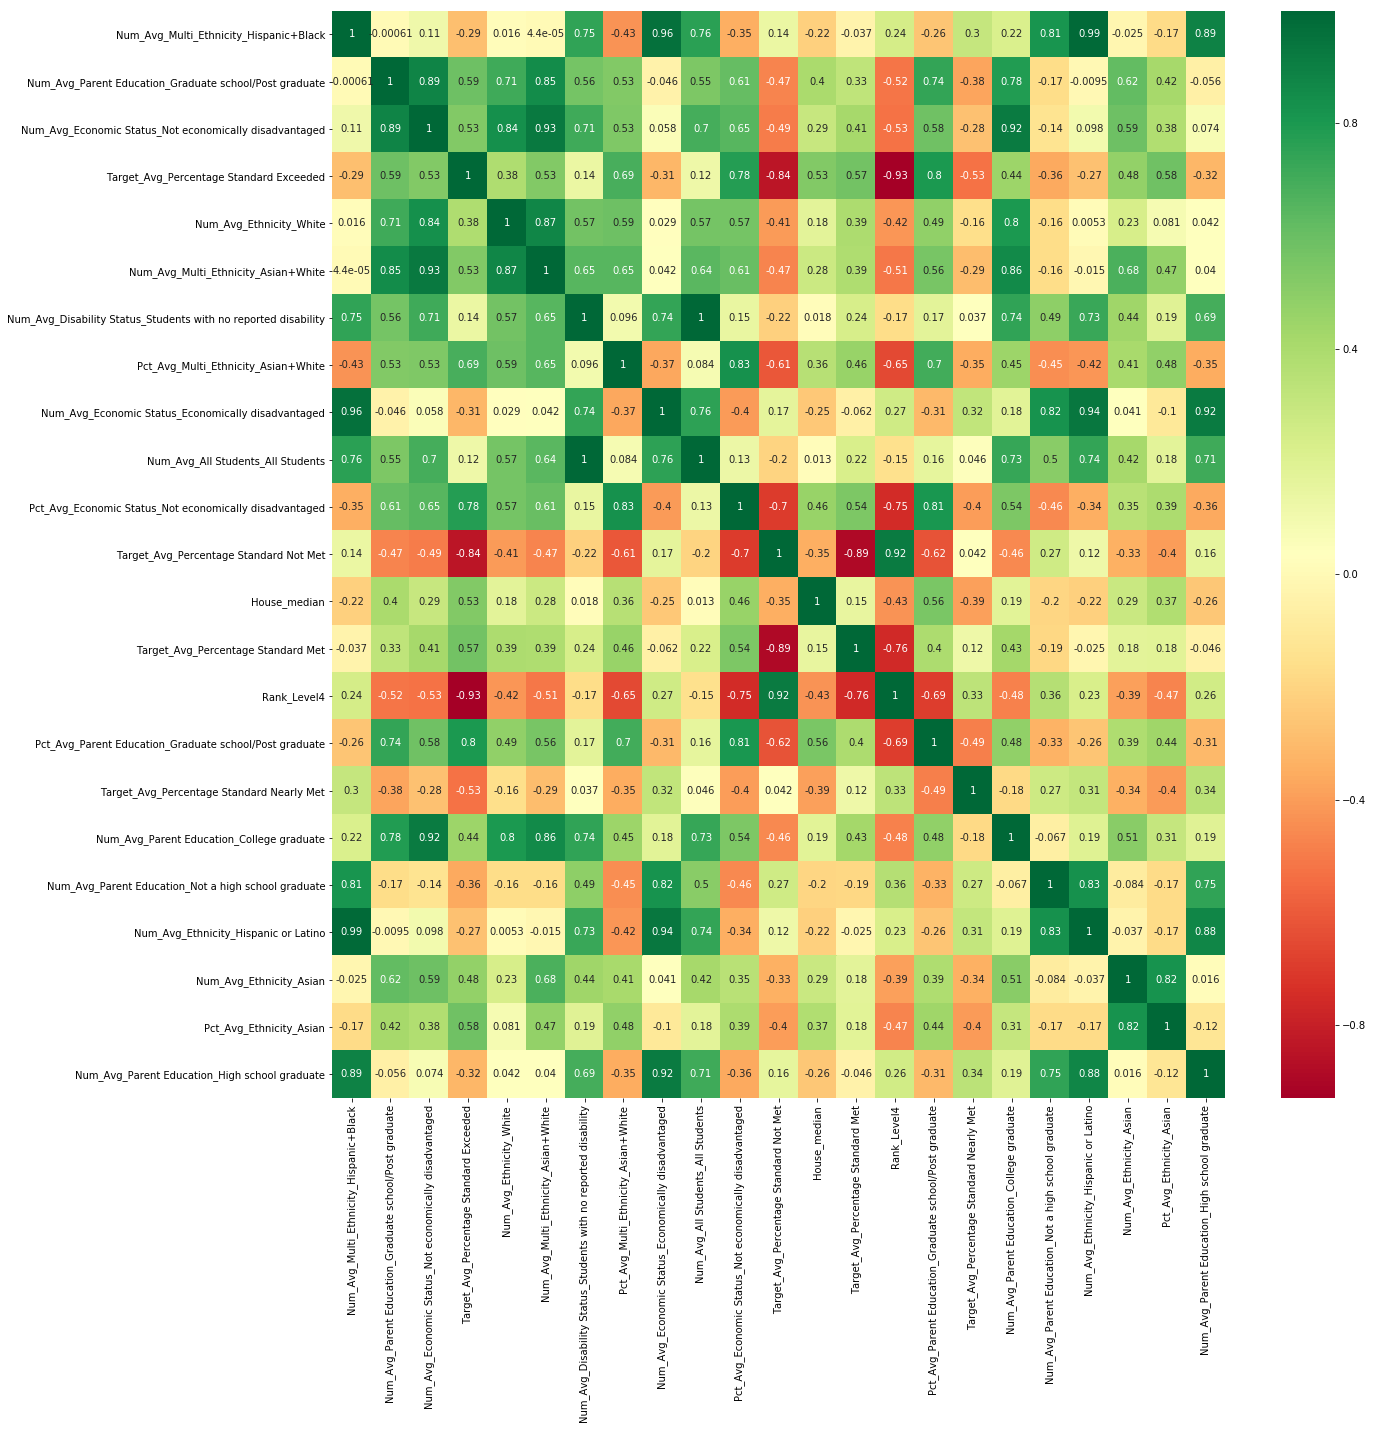
\includegraphics[width=\textwidth]{output_108_0.png}
%\caption{Correlation Table in Specific Inferior Group.}
%  \label{fig:corr_inferior}
%\end{figure}

\subsubsection{Pearson's Correlation Coefficient}

Pearson's correlation coefficient tests whether two samples have a linear relationship.

\noindent \textbf{Assumptions:}\\
- Observations in each sample are independent and identically distributed.
- Observations in each sample are normally distributed.
- Observations in each sample have the same variance.

\noindent \textbf{Interpretation:}\\
\indent - $H_0$: The two samples are independent.\\
\indent - $H_1$: There is a dependency between the samples.

For example, we calculate the Pearson's Correlation Using SciPy, `scipy.stats.pearsonr(x, y)`.  
For example, we investigated the relationship between 'Pct\_Ethnicity\_Asian\_Mathematics' and 'Target\_Percentage Standard Exceeded\_Mathematics' and obtained the results as below.
\begin{verbatim}
* Spearman Rank Correlation between 'Pct\_Ethnicity\_Asian\_Mathematics'
and 'Target\_Percentage Standard Exceeded\_Mathematics':
corr: 0.6111925793, p-value: 0.0000000000
\end{verbatim}
We reject the null hypothesis $H_0$.
The portion of Asian students and the higher scores in Mathematics is \textbf{not independent but strongly correlated}.

\subsubsection{Spearman's Rank Correlation}

Spearman's correlation measures the strength and direction of monotonic association between two variables. Spearman’s rank correlation is the Pearson’s correlation coefficient of the ranked version of the variables. We can define a function for calculating the spearman's rank correlation.

\noindent \textbf{Assumptions:}\\
Observations in each sample are independent and identically distributed. Observations in each sample can be ranked.

\noindent \textbf{Interpretation:}\\
\indent - $H_0$: The two samples are independent.\\
\indent - $H_1$: There is a dependency between the samples.

For example, 
we calculate Spearman’s Rank Correlation Using SciPy, `scipy.stats.spearmanr(x, y)'.
For example, we investigated the relationship between 'House\_median' and 'Target\_Avg\_Percentage Standard Exceeded'.
\begin{verbatim}
* Spearman Rank Correlation between 'House_median' 
and 'Target_Avg_Percentage Standard Exceeded':
corr: 0.4723283465, p-value: 0.0000000000
\end{verbatim}
We reject the null hypothesis $H_0$.
The house prices and high scores is \textbf{not independent but correlated}.

\subsection{Feature Selection}

\subsubsection{Univariate Selection}

Statistical tests can be used to select those features that have the strongest relationship with the output variable.
%
The scikit-learn library provides the \href{https://scikit-learn.org/stable/modules/generated/sklearn.feature_selection.SelectKBest.html#sklearn.feature_selection.SelectKBest}{SelectKBest} class that can be used with a suite of different statistical tests to select a specific number of features.
%
We use the chi-squared (chi$^{2}$) statistical test for non-negative features to select 20 best features.

The best features in the larger order of scores are as follows:
\begin{enumerate}[topsep=0pt,itemsep=-1ex,partopsep=1ex,parsep=1ex]
\item 'House\_median'
\item 'Rank\_Level4'
\item 'Num\_Avg\_Economic Status\_Not economically disadvantaged'
\item 'Num\_Avg\_Multi\_Ethnicity\_Asian+White'
\item 'Num\_Avg\_Parent Education\_Graduate school/Post graduate'
\item 'Num\_Avg\_Ethnicity\_Asian'
\item 'Num\_Avg\_Economic Status\_Economically disadvantaged'
\item 'Num\_Avg\_Multi\_Ethnicity\_Hispanic+Black'
\item 'Num\_Avg\_Ethnicity\_White'
\item 'Num\_Avg\_Ethnicity\_Hispanic or Latino'
\item 'Num\_Avg\_Parent Education\_College graduate'
\item 'Num\_Avg\_Parent Education\_Not a high school graduate'
\item 'Num\_Avg\_All Students\_All Students'
\item 'Num\_Avg\_Disability Status\_Students with no reported disability'
\item 'Pct\_Avg\_Economic Status\_Not economically disadvantaged'
\item 'Pct\_Avg\_Parent Education\_Graduate school/Post graduate'
\item 'Num\_Avg\_Parent Education\_High school graduate'
\item 'Pct\_Avg\_Multi\_Ethnicity\_Asian+White'
\item 'Pct\_Avg\_Ethnicity\_Asian'
\item 'Target\_Avg\_Percentage Standard Not Met'
\end{enumerate}

As expected, for the higher achievement (Percentage of Standard Exceeded), higher house prices, higher economic status, Asians and Whites in Ethnicity, and higher education. `Rank\_Level4' is derived from the Percentage of Standard Exceeded, so it must be strongly correlated.

\subsubsection{Feature Importance}

We obtain the feature importance of each feature of the dataset by using the feature importance property of the model.
%
Feature importance gives you a score for each feature of the data, the higher the score more important or relevant is the feature towards the output variable.
%
Feature importance is an inbuilt class that comes with Tree Based Classifiers, we used the Extra Tree Classifier for extracting the top 20 features for the dataset.

\begin{figure}[h!]
\centering 
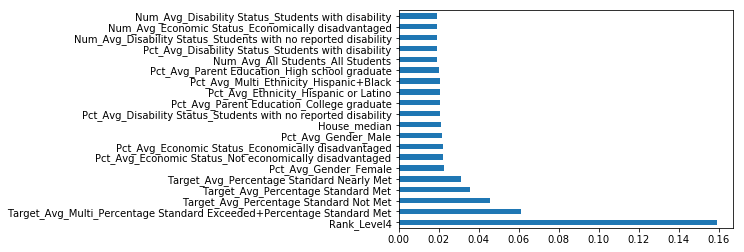
\includegraphics[width=\textwidth]{output_102_1.png}
\caption{Feature importance using Extra Tree Classifier for extracting the top 20 features.}
  \label{fig:feature_importance_top20}
\end{figure}

As can be seen in Figure \ref{fig:feature_importance_top20}, the `Rank\_Level4'
 and the other score variables are identified as the important features.

%Finally, we identify the important features as below. These features will be used for building machine learning models later.

%\subsection{Data Preprocessing}

\subsection{Variables for Modeling}
\label{Variables for Modeling}

\paragraph*{Newly Derived Variables.}

For independent variable, 
we add new variables by combining Asian and Whites as well as Hispanic and Black students in the Ethnicity, so we expect this addition to tell new insights.
%
In addition, we merge variables for ``Native Hawaiian or Pacific Islander" and ``American Indian or Alaska Native" for the minor groups of ethnicity, so we expect this merging can reduce the dimensionality.

%
For target variables, we created the label "NeedHelp". The school is encoded to 1 when the 'Percentage Standard Not Met' $>$ 80\%, otherwise 0.
%
The 312 schools have been identified to this inferior group, while only 8 schools have been found when the 'Percentage Standard Exceeded' $>$ 80\%.
%
By analyzing the inferior group, many of those schools have zero percent of 'Percentage of Standard Exceeded' students.

\subsubsection{Independent variables}

We summarize the independent variables as follows.\\
\noindent \textbf{Organized variables:}\\ 
- [`Num'] x [`Category' + `Student Groups' + `Test Id']: \\
\indent    - `Num': `Students with Scores' (Number of students)\\
\indent    - `Test Id' = [English, Mathematics]\\
\indent    - `Category' and `Student Groups': (47 student category groups in Table \ref{table:student_group}.)\\
- House\_median: House median prices in the school zones
    
\noindent \textbf{New variables:}\\ 
- [`Pct'] x [`Category' + `Student Groups' + `Test Id']:\\ 
 \indent   - `Pct': Percentage of students over all students in a school\\
- ([`Num`] $|$ [`Pct']) x [`Avg' + `Category' + `Student Groups']:\\
\indent    - 'Avg' means the average number of percentage of students for English and Mathematics, \\
\indent - `Avg' = (English + Mathematics) / 2\\
- ['Pct'] x (['Multi' + 'Test Id'] or ['Avg' + 'Multi']):\\
\indent    - 'Multi':\\
\indent \indent        - 'Asian+White' or 'Hispanic+Black' in 'Ethnicity'\\
\indent \indent        - `Minor' indicates `American Indian or Alaska Native' and `Native Hawaiian or Pacific Islander'

\subsubsection{Dependent Variable}
%\noindent \textbf{Target variable (Dependent variable):}\\
Then, we set a target variable, e.g., 'Percentage Standard Exceeded' or 'Percentage Standard Not Met', to be investigated. We are interested in the group of students whose performance achievements are exceeded or too inferior. By knowing the characteristics affecting those groups, we can make a score prediction and suggest recommendations later.
We summarize the target variables as follows.

\noindent \textbf{Continuous:}\\
- Average percentage (Target\_Avg) for all four achievement levels:\\
\indent - `Percentage Standard Exceeded': Exceeded (Level 4)\\
\indent    - `Percentage Standard Met': Standard (Level 3)\\
\indent    - `Percentage Standard Nearly Met': Nearly (Level 2)\\
\indent    - `Percentage Standard Not Met': NotMet (Level 1) \\ 
- ['Target\_Avg\_Multi\_Percentage Standard Exceeded+Percentage Standard Met']:\\
\indent   - Sum of two levels (Level 4 + Level 3) that can represent the portions that achieve the standards in a school.\\
%
\textbf{Ordinal:}\\
- 'Rank\_Level4': ranked in a descending order for scores of 'Percentage Standard Exceeded' (Level 4). In short, the 1st indicates the top school.\\
- 'Rank\_Level1': ranked in a descending order for scores of 'Percentage Standard Not Met' (Level 
1). In short, the 1st indicates the inferior school.\\
%
\textbf{Categorical:}\\
- `Need Help' [1] ('Percentage Standard Not Met' $>$ 80\%) / `No Need Help' [0] (others) labels (for Classification)

\section{Modeling}
\label{Modeling}

The aim is to predict the inferior scores (i.e., percentage of the standard "NOT" met) of schools. 
We used the supervised machine learning  algorithms including the regression and classification to build predictive models.
%
Based on these prediction models, we can 1) identify the schools that need help and 2) obtain important features affecting the lower scores of schools. 
%
More details with codes on machine learning modeling can be found in
\href{https://github.com/ahrimhan/data-science-project/blob/master/project1/machine_learning.ipynb}{this IPython notebook}. 

\subsection{Regression}

Regression analysis is a subfield of supervised machine learning. It aims to model the relationship between a certain number of features and a continuous target variable.
%
In the regression, we use the `Target\_Avg\_Percentage Standard Not Met` variable as a target variable. 

\subsubsection{Cross Validation: Train/Test Split, Leave One Out (LOO), K-Fold CV}

We need to split the data into training and testing sets, fitted a regression model to the training data, made predictions based on this data and tested the predictions on the test data using the \href{https://scikit-learn.org/stable/modules/cross_validation.html}{cross validation}. 

However, the \href{https://towardsdatascience.com/train-test-split-and-cross-validation-in-python-80b61beca4b6}{train/test split technique} takes to one extreme, $K$ may be set to 1 such that a single train/test split is created to evaluate the model. Thus, the \textbf{train/test split technique is not stable in that it may not split the data randomly and the data can be selected only from specific groups.} This will result in overfitting.

The Leave One Out Cross Validation (LOOCV) takes to another extreme, $K$ may be set to the total number of observations in the dataset such that each observation is given a chance to be the held out of the dataset. This is called leave-one-out cross-validation, or LOOCV for short. However, \textbf{LOO requires quite a large computation time.}

\textbf{Therefore, we the cross validations: K-Fold.} This \href{https://machinelearningmastery.com/k-fold-cross-validation/}{K-Fold cross validation} is enough and appropriate for our model prediction.

\subsubsection{Evaluation Metrics: MAE, RMSE, and R$^{2}$}

\begin{itemize}
	\item Mean Absolute Error (MAE): MAE is the mean of the absolute value of the errors. 
\item Root Mean Squared Error (RMSE): RMSE is the square root of the mean of the squared errors
\item R$^{2}$: R$^{2}$ is the number that indicates the proportion of the variance in the dependent variable that is predictable from the independent variables. Basically, R$^{2}$ represents how accurate our model is. R$^{2}$ shows how well terms (data points) fit a curve or line. Adjusted R$^{2}$ also indicates how well terms fit a curve or line, but adjusts for the number of terms in a model. 
\end{itemize}

\subsubsection{Algorithms: Linear Regression, Random Forest Regressor, Gradient Boosting Regressor}
\label{Regression_algorithms}

\paragraph*{Linear Regression:}
Linear regression attempts to model the relationship between two variables by fitting a linear equation to observed data. One variable is considered to be an explanatory variable, and the other is considered to be a dependent variable. 

When the outcome we are trying to predict depends on more than one variable, we can make the \href{https://towardsdatascience.com/supervised-learning-basics-of-linear-regression-1cbab48d0eba}{multiple linear regression model} which is more complicated model that takes this higher dimensionality into account. As long as they are relevant to the problem faced, using more predictor variables can help us to get a better prediction.

\begin{itemize}
	\item \textbf{Train/Test Split Cross Validation for Linear Regression:} For a simple example, we split data into 70\% train and 30\% test data. Out of 8,768 instances with 40 features, 6,137 is train data and 2,631 is test data.
% 
We fit the model and present the coefficients of the regression model. 

Figure \ref{fig:reg_coef_traintestsplit} represents the sorted the coefficients in a descending order of absolute values. 
The major affecting features for predicting the percentage of the standard "NOT" met schools are 
the number of Black or Hispanic students.

\begin{figure}[h!]
\centering 
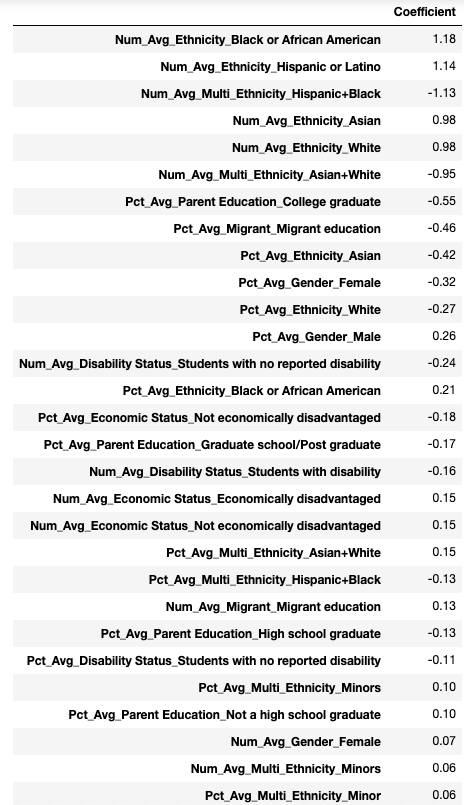
\includegraphics[scale=0.6]{reg_coef_traintestsplit.png}
\caption{Coefficients of the regression model with train (70\%) and test (30\%) split data.}
  \label{fig:reg_coef_traintestsplit}
\end{figure}

The results of the train and test split for Linear Regression model are as follows:
RMSE:  11.2853, MAE:  8.2113, and R$^{2}$ score: 0.6614.

\item \textbf{Leave One Out Cross Validation (LOOCV) for Linear Regression:}
The results of the \textit{leave one out} cross validated (number of splits: 8,768) Linear Regression model are as follows:
RMSE:  11.3417 and MAE:  8.2913.

\item \textbf{10-Fold Cross Validation for Linear Regression:}
After fitting a model, we plotted the actual values (X-axis) and predicted values (Y-axis) (Figure \ref{fig:reg_plot_10fold}).
%
The results of the 10 fold cross validated Linear Regression model are as follows:
%
RMSE:  11.7262, MAE:  8.5554, and R$^{2}$ score:  0.6233.

\begin{figure}[h!]
\centering 
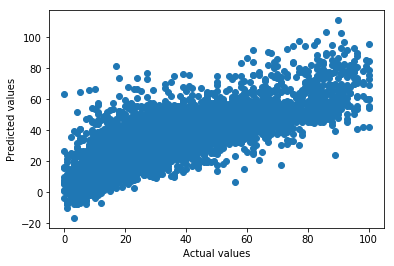
\includegraphics[scale=0.5]{reg_plot_10fold.png}
\caption{Plotted actual and predicted values using the Linear Regression with 10-fold Cross Validation.}
  \label{fig:reg_plot_10fold}
\end{figure}

\end{itemize}

\paragraph*{Random Forest Regressor:}
A random forest is a meta estimator that fits a number of classifying decision trees on various sub-samples of the dataset and uses averaging to improve the predictive accuracy and control over-fitting. The sub-sample size is always the same as the original input sample size but the samples are drawn with replacement if bootstrap = True (default).
%
The results of the 10 fold cross validated Random Forest Regressor model are as follows:
RMSE:  10.7661, MAE:  7.6911, and R$^{2}$ score:  0.6763.

\paragraph*{Gradient Boosting Regressor:}
GB builds an additive model in a forward stage-wise fashion; it allows for the optimization of arbitrary differentiable loss functions. In each stage a regression tree is fit on the negative gradient of the given loss function.
%
The results of the 10 fold cross validated Gradient Boosting for Regression model are as follows:
RMSE:  11.4108, MAE:  8.3881, and R$^{2}$ score:  0.6368.

\subsubsection{Results of Regression}

The results of the accuracy for regression models is summarized in Table \ref{table:acc_regression}. The \textbf{Random Forest Regressor worked best} with Root Mean Squared Error (RMSE) 10.7672, Mean Absolute Error (MAE) 7.6985, and R$^{2}$ 0.6761.

\begin{table}[h]
\centering
\begin{tabular}{||c|c|c|c||}
  \hline
Model Name & RMSE & MAE & R$^{2}$\\
  \hline
Linear Regression with 1 folds Train and test split & 11.2853 &  8.2113 & 0.6614\\
\hline
Linear Regression with 8,768 folds Leave One Out (LOO) & 11.3417 & 8.2913 & 0.0000\\
\hline
Linear Regression with 10 folds CV & 11.7262 & 8.5554 &  0.6233\\
\hline
\cellcolor{red!25}Random Forest Regressor with 10 folds CV & \cellcolor{red!25}10.7661 & \cellcolor{red!25}7.6911 &  \cellcolor{red!25}0.6763\\
\hline
Gradient Boosting for Regression with 10 folds CV & 11.4108 & 8.3881 & 0.6368\\
  \hline
\end{tabular}
\caption{Results of the accuracy for regression models.}
\label{table:acc_regression}
\end{table}

\subsection{Classification}

\subsubsection{Preprocessing Data and Stratified K-Folds Cross Validation}

\paragraph*{Preprocessing Data.\\}

\noindent \textbf{New Binary Target Variable (`NeedHelp'):} We use the `NeedHelp` variable as a target variable. The variables used for modeling are explained in Section \ref{Variables for Modeling}.
%
Given the brief explanation, the `NeedHelp' indicates that if a school needs help or not. We have labeled schools with more than 80\% of students who do not meet the standard as needing help (1), otherwise (0).

\noindent \textbf{Resolving Imbalanced Classes:} We observed that the `NeedHelp` has imbalanced classes: 3.69\% of our dataset belong to the target class `NeedHelp`.
%
To overcome the problem of the \textbf{imbalanced classes}, we need to deal with this imbalanced classes properly: 1) Stratified K-Folds Cross Validation and 2) weighted evaluation metrics to reflect the mass of the classes.

\noindent \textbf{Data Splitting into Train Data and Test Data:}
We basically split data into train data and test data into the ratio of 70\% and 30\%. For parameter tuning, we use the cross validation in the train data and build the machine learning model, then validate the model with the remained test data. This more detailed explanation is given in Section \ref{Classification_algorithms} in Figure \ref{fig:grid_search_cross_validation}. 

\noindent \textbf{Scaling:} For the K-Nearest Neighbor algorithm, we scale the independent variables (X\_train and X\_test) into the  
range such that the range is now between 0 and 1. 
%
If the distribution is not Gaussian or the standard deviation is very small, the min-max scaler works better than standard scaler.

\paragraph*{Cross Validation: Stratified K-Folds Cross Validation.}

We used the `Stratified K-Folds Cross Validation` \cite{stratified_cv}.
This cross-validation object is a variation of KFold that returns stratified folds. The folds are made by preserving the percentage of samples for each class. In short, the stratification will ensure that the percentages of each class in your entire data will be the same (or very close to) within each individual fold.  

\subsubsection{Evaluation Metrics: Accuracy, AUC, Precision, Recall, F1}

We use the weighted option when calculating the precision, recall, and f1 scores to reflect the mass of the classes.
It calculates metrics for each label and finds their average weighted by support (the number of true instances for each label). This alters 'macro' to account for label imbalance; it can result in an F-score that is not between precision and recall.
%
We also present the Receiver Operating Characteristic (ROC) curve and Area Under the Curve (AUC). 


\subsubsection{Algorithms: Logistic Regression, Decision Tree, GridSearchCV for Parameter Tuning for Decision Tree, Random Forest Classifier, and k-Nearest Neighbors Classifier}
\label{Classification_algorithms}

\paragraph*{Logistic Regression:}
Logistic regression is the appropriate regression analysis to conduct when the dependent variable is dichotomous (binary). Logistic regression is used to describe data and to explain the relationship between one dependent binary variable and one or more nominal, ordinal, interval or ratio-level independent variables.

\begin{itemize}
\item \textbf{Train/Test Split Cross Validation for Logistic Regression:}
Figure \ref{fig:clf_logistic_split_result} shows the results of the Logistic Regression with train (70\%) and test (30\%) split data.
%
\begin{figure}[h]
\centering 
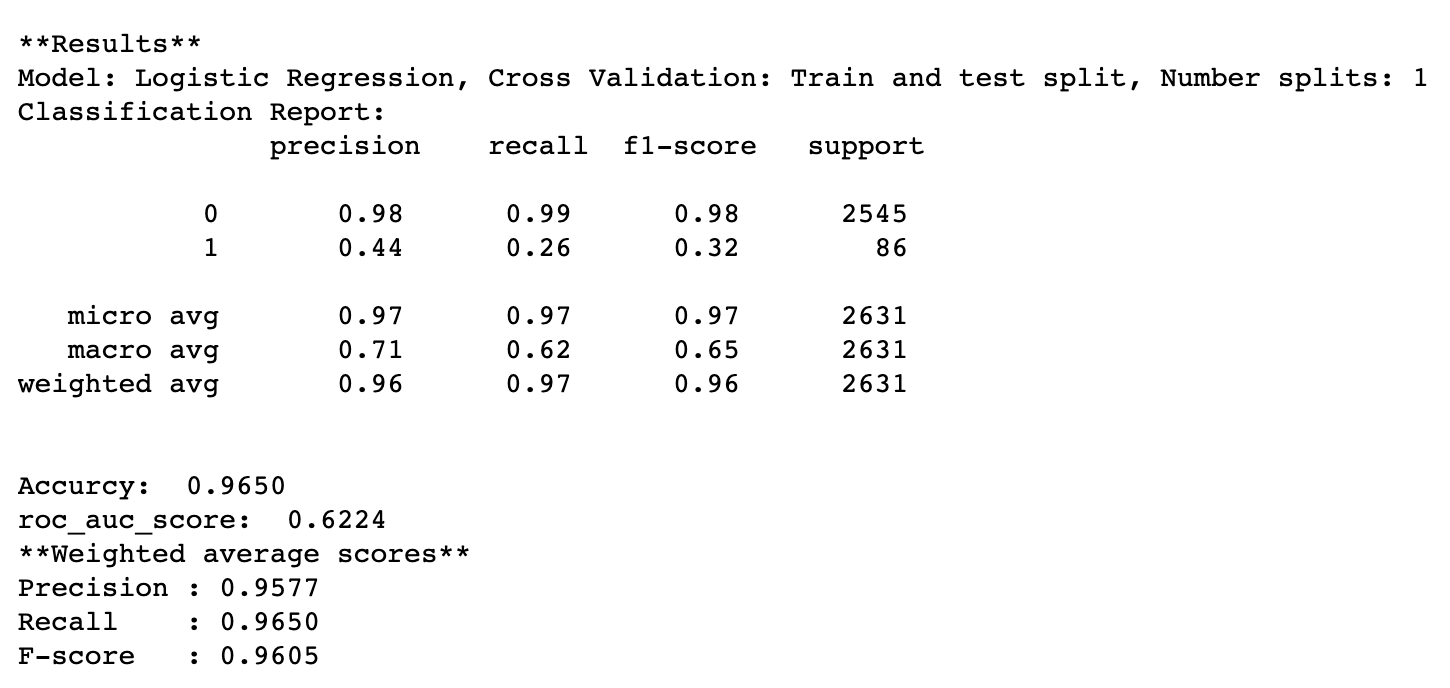
\includegraphics[scale=0.5]{clf_logistic_split_result.png}
\caption{Logistic Regression with train and test split data.}
  \label{fig:clf_logistic_split_result}
\end{figure}

\item \textbf{Stratified 5-Folds Cross Validation for Logistic Regression:}
Figure \ref{fig:clf_logistic_5fold} represents the results of the Logistic Regression with Stratified 5-Folds CV.
%
The results model evaluation are as follows:
accuracy: 0.9656,
roc\_auc\_score: 0.9656,
weighted avg precision: 0.9646,
weighted avg recall: 0.9656, and
weighted avg f1-score: 0.9597.

\begin{figure}[h!]
\centering
\begin{subfigure}{0.5\textwidth}
         \centering
         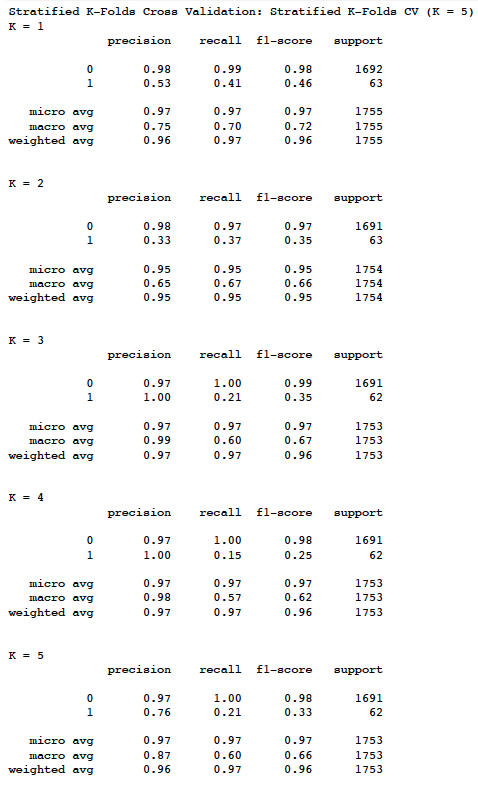
\includegraphics[width=\textwidth]{clf_logistic_5fold.png}
         \caption{Each Fold in Stratified 5-Fold CV.}
         \label{fig:clf_logistic_5fold}
\end{subfigure}
\hfill
\begin{subfigure}{0.6\textwidth}
         \centering
         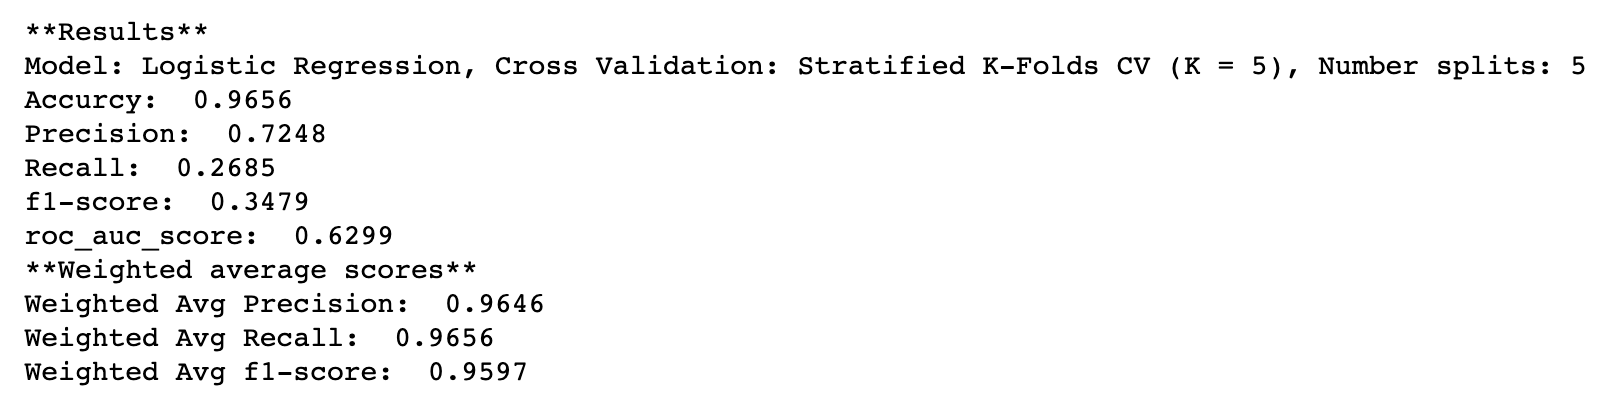
\includegraphics[width=\textwidth]{clf_logistic_5fold_result.png}
         \caption{Mean results of 5-fold Cross Validated Logistic Regression.}
         \label{fig:clf_logistic_5fold_result}
\end{subfigure}
\caption{Results of the Logistic Regression with Stratified 5-Folds CV.}
\label{fig:clf_logistic_5fold}
\end{figure}
\end{itemize}

%============================%
\paragraph*{Decision Tree:}
The decision tree classifier iteratively divides the working area (plot) into subpart by identifying lines.
There are three key terms related to decision tree classifiers:

\noindent \textbf{Criterion}
\begin{itemize}
\item Impurity:  
Impurity is when we have a traces of one class division into other.
\item Entropy:  
Entropy is a degree of randomness of elements. In other words, it is a measure of impurity. It is the negative summation of probability times the log of the probability of item x.
\item Information gain:  
Information Gain (n) = Entropy(x) — ([weighted average] * entropy(children for feature)) \\
At every stage, a decision tree selects the one that gives the best information gain. An information gain of 0 means the feature does not divide the working set at all.
\end{itemize}

%
\textbf{\href{https://www.datacamp.com/community/tutorials/decision-tree-classification-python}{Optimizing Decision Tree Performance}}
\begin{itemize}
\item criterion : optional (default=”gini”) or Choose attribute selection measure: This parameter allows us to use the different-different attribute selection measure. Supported criteria are “gini” for the Gini index and “entropy” for the information gain.
\item splitter : string, optional (default=”best”) or Split Strategy: This parameter allows us to choose the split strategy. Supported strategies are “best” to choose the best split and “random” to choose the best random split.
\item max\_depth : int or None, optional (default=None) or Maximum Depth of a Tree: The maximum depth of the tree. If None, then nodes are expanded until all the leaves contain less than min\_samples\_split samples. The higher value of maximum depth causes overfitting, and a lower value causes underfitting (Source).
\end{itemize}
%

\begin{itemize}
\item \textbf{Stratified 5-Folds Cross Validation for Decision Tree:}
The Figure 
Figure \ref{fig:dtree_cv} represents the results of the Decision Tree with Stratified 5-Folds CV.%
%
The results model evaluation are as follows:
accuracy: 0.9596,
roc\_auc\_score: 0.7320,
weighted avg precision: 0.9660,
weighted avg recall: 0.9596, and
weighted avg f1-score: 0.9614.

\begin{figure}[h!]
\centering
\begin{subfigure}{0.6\textwidth}
         \centering
         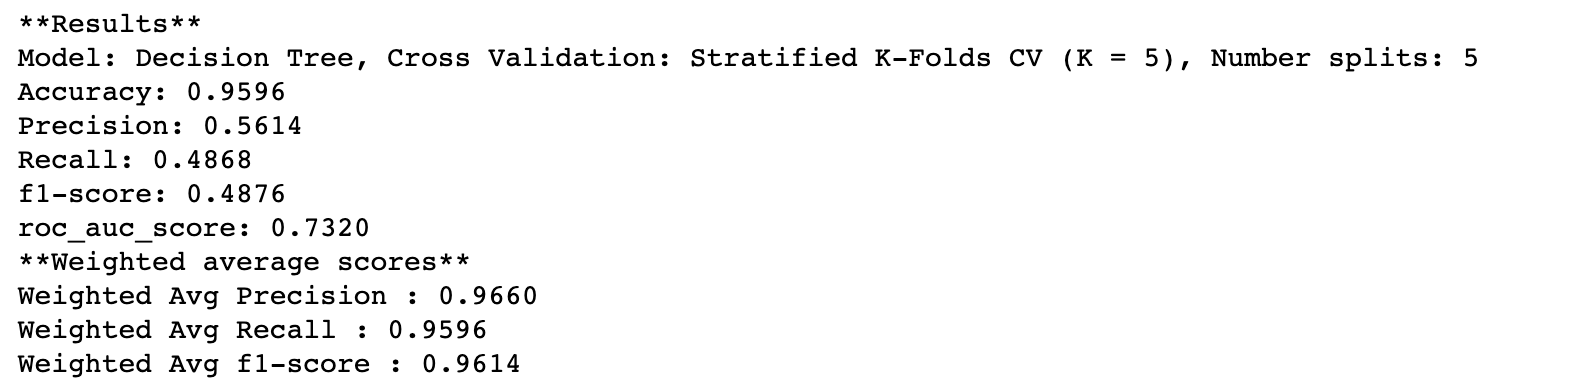
\includegraphics[width=\textwidth]{dtree_cv.png}
         \caption{Result}
         \label{fig:dtree_cv_report}
\end{subfigure}
\hfill
\begin{subfigure}{0.38\textwidth}
         \centering
         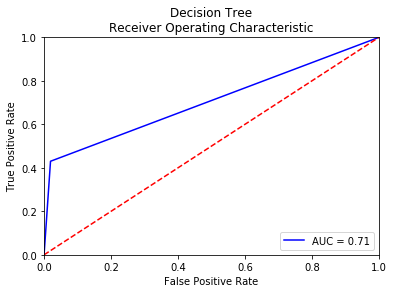
\includegraphics[width=\textwidth]{dtree_cv_auc.png}
         \caption{AUC graph}
         \label{fig:dtree_cv_auc}
\end{subfigure}
\caption{Results of the Decision Tree with Stratified 5-Folds CV.}
\label{fig:dtree_cv}
\end{figure}
\end{itemize}


\paragraph*{GridSearchCV for Parameter Tuning:}
The grid search cross validation for parameter tuning process is as follows (see Figure \ref{fig:grid_search_cross_validation}). We first split the train data and test data in the ratio of 70\% and 30\%. In the train data, we use the k-fold cross validation for finding (tuning) the parameters. After the finding parameter process is finished, we use the remained test data to evaluate the model.

Using the `GridSearchCV` for parameter tuning can be burden in the aspect of time and computation.
%
For example, for a model, if we consider 10-fold validation, 3 parameters in which one of each has 5 values, then the model needs to be run 1,250 (= 5 * 5 * 5 * 10) times.
%

\begin{figure}[h]
\centering 
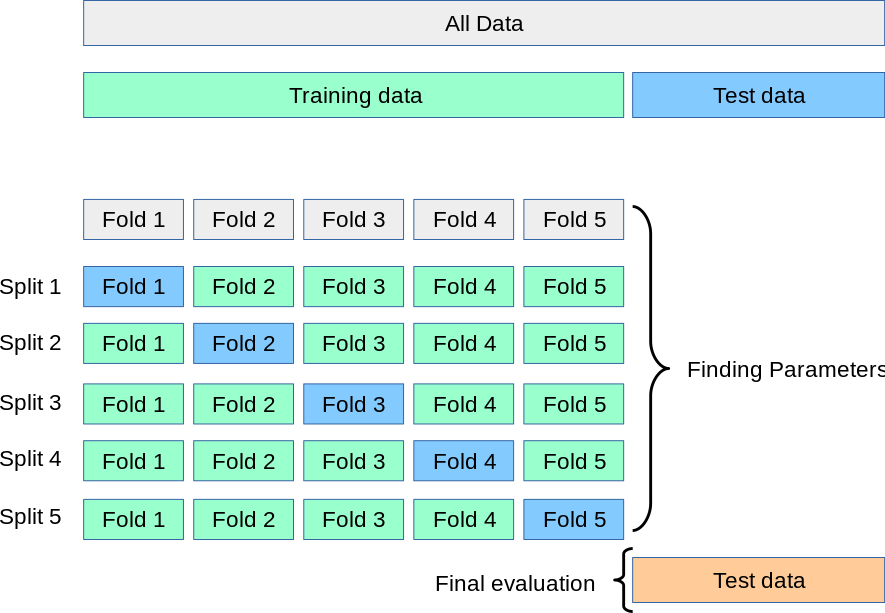
\includegraphics[width=\linewidth]{grid_search_cross_validation.png}
\caption{Grid Search Cross Validation for Parameter Tuning using Training Set and Final Evaluation using Test Set \cite{gridsearchcv}.}
  \label{fig:grid_search_cross_validation}
\end{figure}

%===================%
\begin{itemize}
\item \textbf{Decision Tree with GridSearchCV:}
Figure \ref{fig:dtree_gridcv} presents 
the results of Decision Tree with Grid Search Cross Validation (Stratified 5-Folds CV) with the following 
parameters: \{'max\_depth': [50, 75, 100], 'min\_samples\_leaf': [1, 2, 4, 8, 10]\}.
%
Here is the best parameters for the Decision Tree model: \{'max\_depth': 50, 'min\_samples\_leaf': 8\}.
The results model evaluation are as follows:
best accuracy: 0.9684,
best roc\_auc\_score: 0.9070,
weighted avg precision: 0.9666,
weighted avg recall: 0.9684, and
weighted avg f1-score: 0.9674.

%Probability Predictions  
Please note that when obtaining the ROC and AUC,
we used the \texttt{predict\_prob} for the prediction of 
the probability of the data instance belonging to each class.
This is called a probability prediction where given a new instance, the model returns the probability for each outcome class as a value between 0 and 1.

%
\begin{figure}[h!]
\centering
\begin{subfigure}{0.6\textwidth}
         \centering
         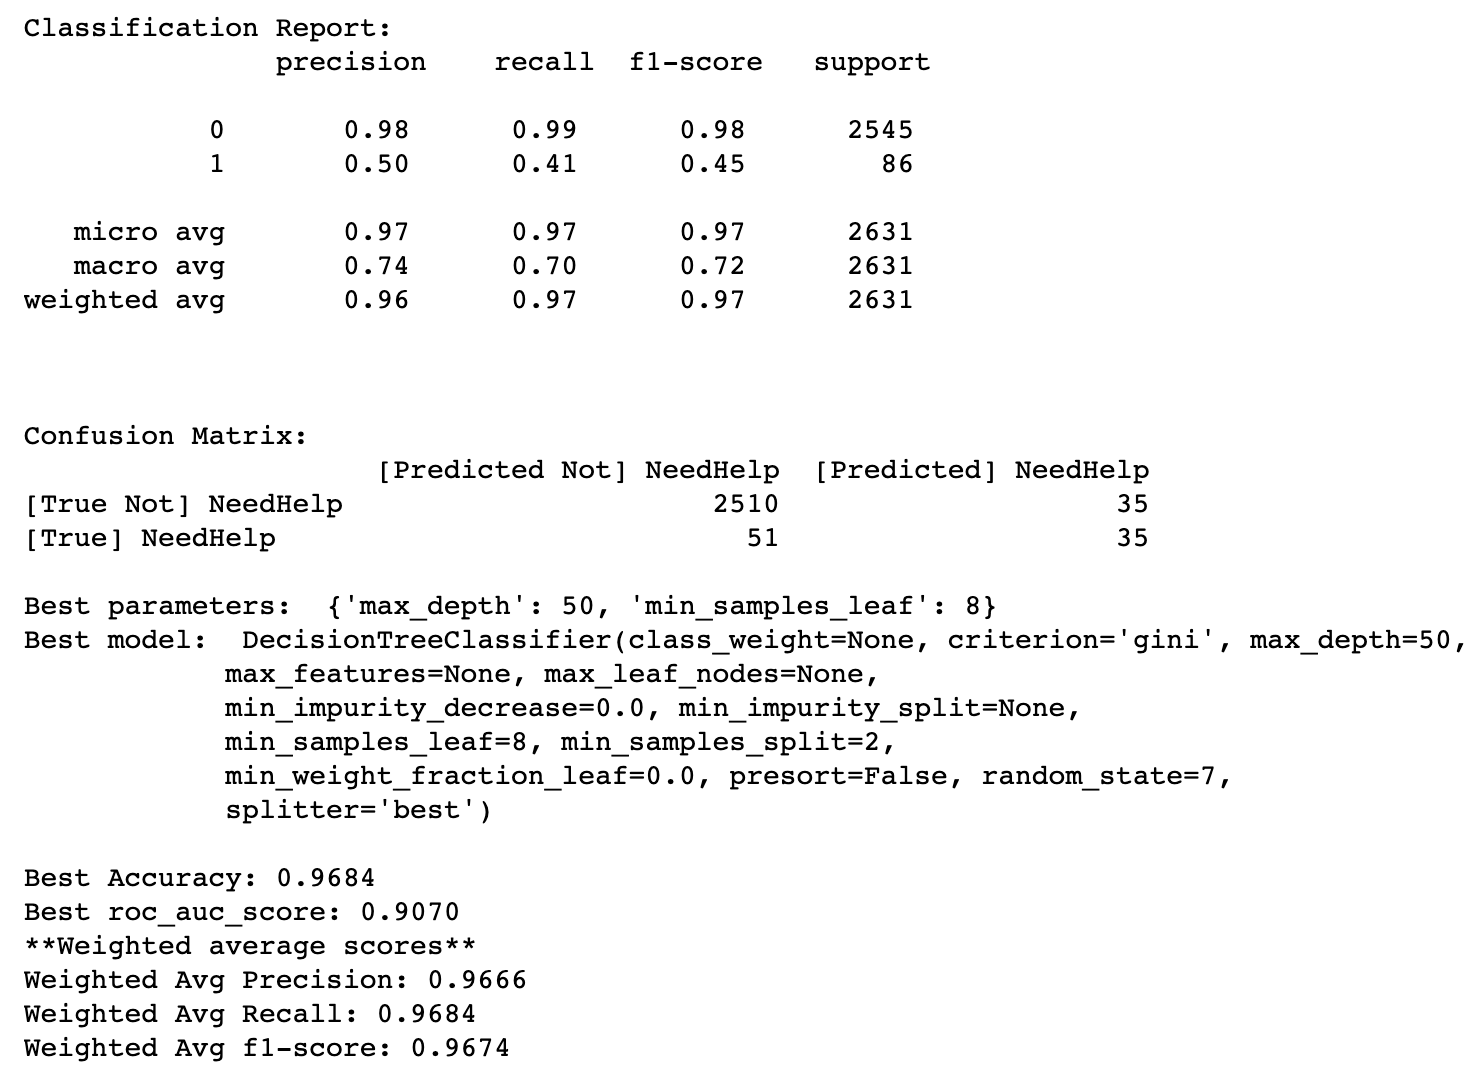
\includegraphics[width=\textwidth]{dtree_gridcv.png}
         \caption{Result}
         \label{fig:dtree_cv_report}
\end{subfigure}
\hfill
\begin{subfigure}{0.38\textwidth}
         \centering
         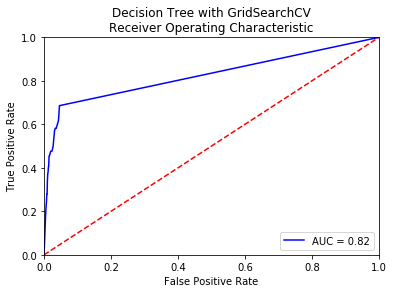
\includegraphics[width=\textwidth]{dtree_gridcv_auc.png}
         \caption{AUC graph}
         \label{fig:dtree_cv_auc}
\end{subfigure}
\caption{Results of the Decision Tree with GridSearchCV.}
\label{fig:dtree_gridcv}
\end{figure}


\textbf{Decision Tree Visualization:}
To have the insights from the selected features used for constructing, we visualize the best Decision Tree in Figure \ref{fig:decison_tree_graphic}.
The blue nodes and the orange nodes represent the "NeedHelp" nodes and the "Not NeedHelp" nodes, respectively.

\begin{figure}[h]
\centering 
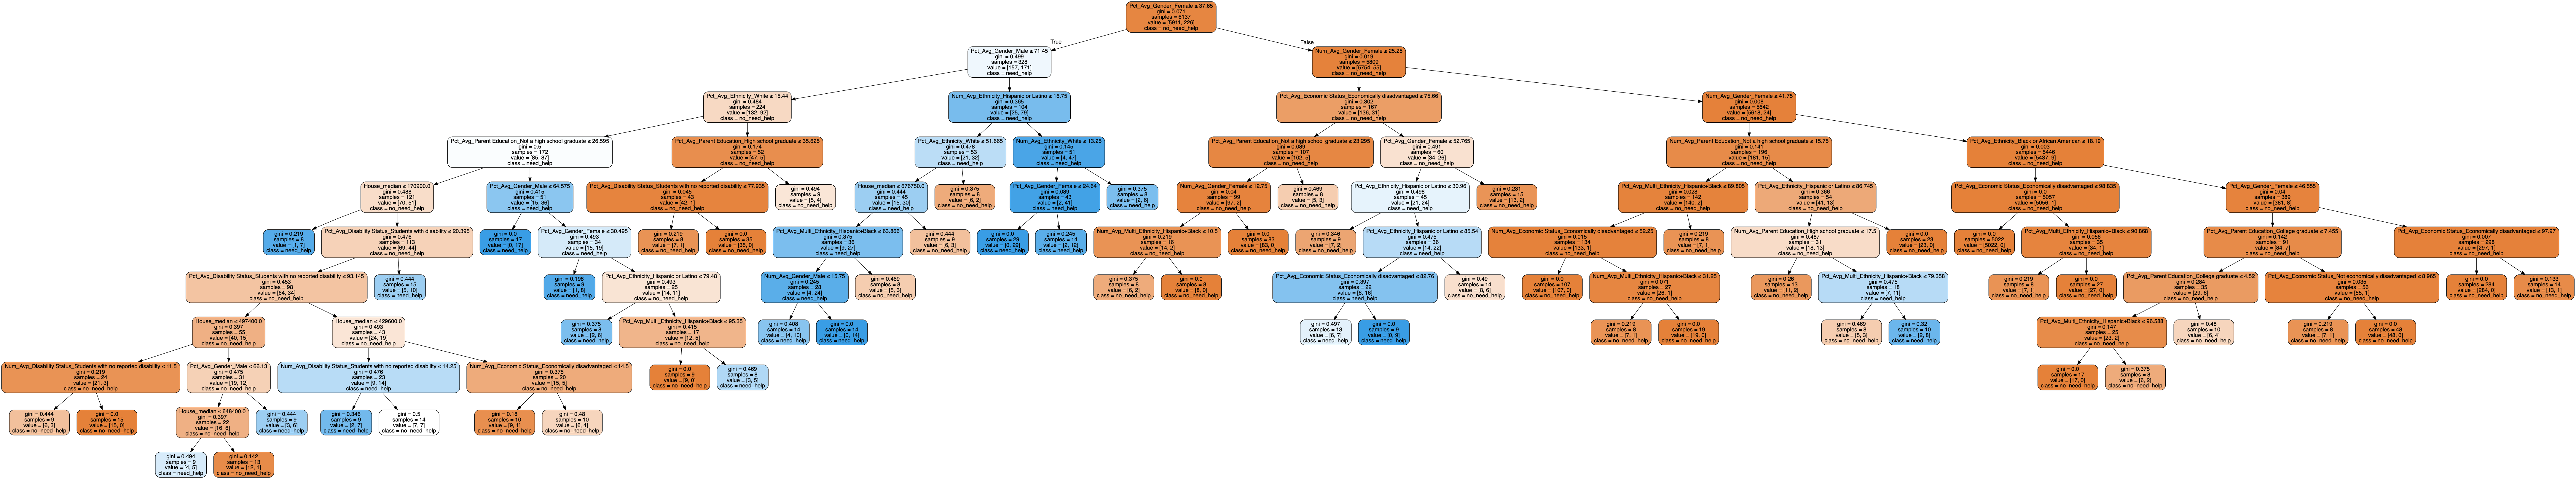
\includegraphics[width=\linewidth]{decison_tree_graphic.png}
\caption{Result of the constructed Decision Tree.}
  \label{fig:decison_tree_graphic}
\end{figure}

\item \textbf{Random Forest Classifier with GridSearchCV:}
Figure \ref{fig:randomforest_gridcv} presents 
the results of Random Forest Classifier with Grid Search Cross Validation (Stratified 5-Folds CV) with the following 
parameters: \{'n\_estimators': [100, 150, 200], 'max\_depth': [100, 150, 200], 'min\_samples\_leaf': [1, 2, 4]\}.
%
Here is the best parameters for the Random Forest Classifier model: 
\{'max\_depth': 100, 'min\_samples\_leaf': 1, 'n\_estimators': 200\}.
%
The results model evaluation are as follows:
best accuracy: 0.9733,
best roc\_auc\_score: 0.9774,
weighted avg precision: 0.9711,
weighted avg recall: 0.9733, and
weighted avg f1-score: 0.9718.
%
\begin{figure}[h]
\centering
\begin{subfigure}{0.6\textwidth}
         \centering
         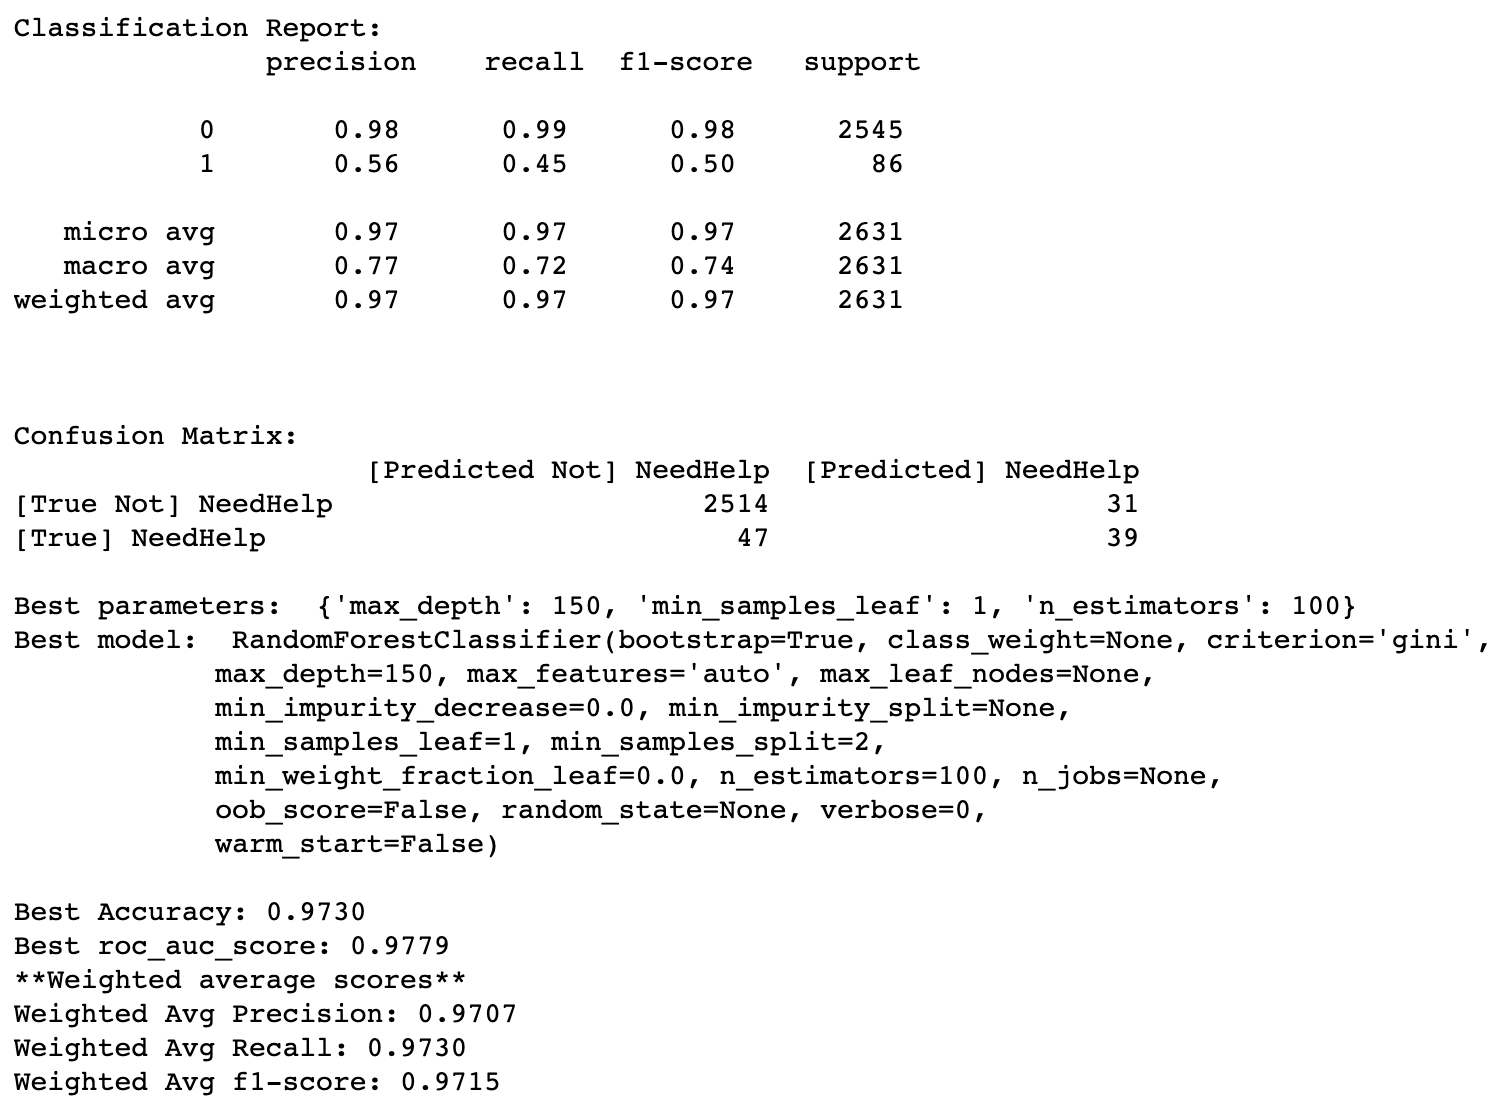
\includegraphics[width=\textwidth]{randomforest_gridcv.png}
         \caption{Result}
         \label{fig:randomforest_gridcv_report}
\end{subfigure}
\hfill
\begin{subfigure}{0.38\textwidth}
         \centering
         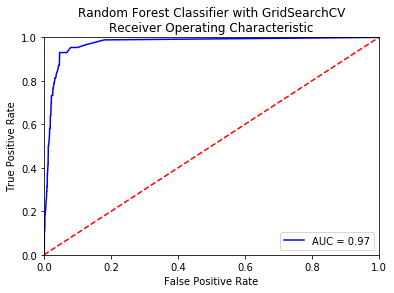
\includegraphics[width=\textwidth]{randomforest_gridcv_auc.png}
         \caption{AUC graph}
         \label{fig:randomforest_gridcv_auc}
\end{subfigure}
\caption{Results of the Random Forest Classifier with GridSearchCV.}
\label{fig:randomforest_gridcv}
\end{figure}

\item \textbf{K-Nearest Neighbor with GridSearchCV (No Scaling):}\\
%
Figure \ref{fig:knear_gridcv_noscale} presents 
the results of K-Nearest Neighbor without scaling with Grid Search Cross Validation (Stratified 5-Folds CV) with the following 
parameters: \{'n\_neighbors': [1, 3, 5, 7, 9, 11, 13, 15, 17, 19, 21, 23, 25, 27, 29], 'weights': ['uniform', 'distance'], 'metric': ['euclidean', 'manhattan']\}.
%
Here is the best parameters for the K-Nearest Neighbor: 
\{'metric': 'manhattan', 'n\_neighbors': 11, 'weights': 'distance'\}.
%
The results model evaluation are as follows:
best accuracy: 0.9650,
best roc\_auc\_score: 0.7309,
weighted avg precision: 0.9556,
weighted avg recall: 0.9650, and
weighted avg f1-score: 0.9526.
%
\begin{figure}[h]
\centering
\begin{subfigure}{0.6\textwidth}
         \centering
         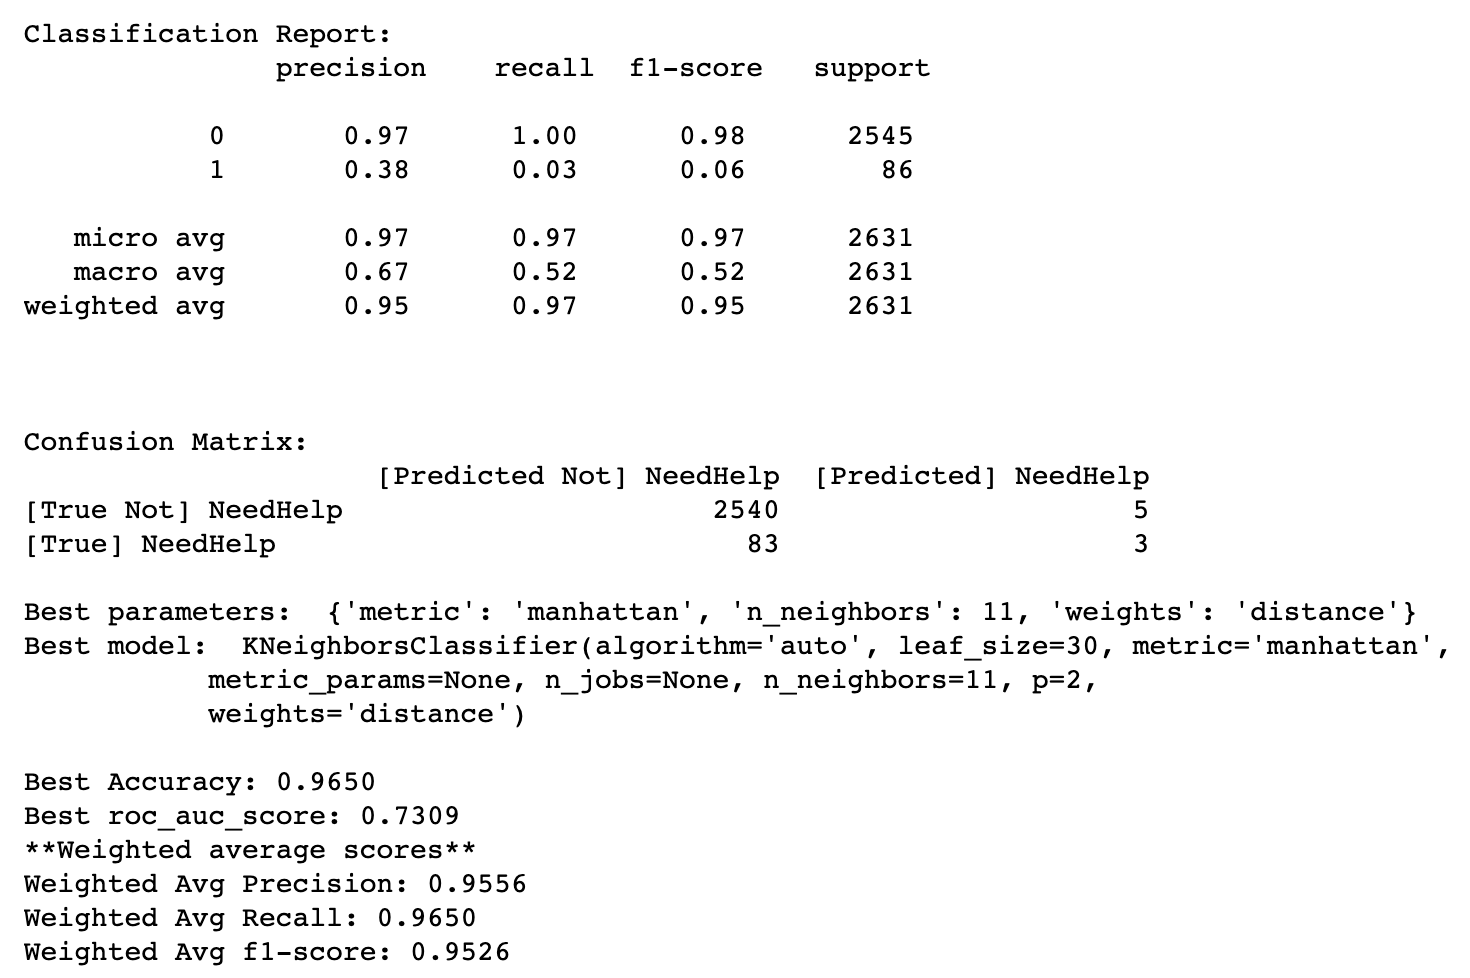
\includegraphics[width=\textwidth]{knear_gridcv_noscaling.png}
         \caption{Result}
         \label{fig:knear_gridcv_noscale_report}
\end{subfigure}
\hfill
\begin{subfigure}{0.38\textwidth}
         \centering
         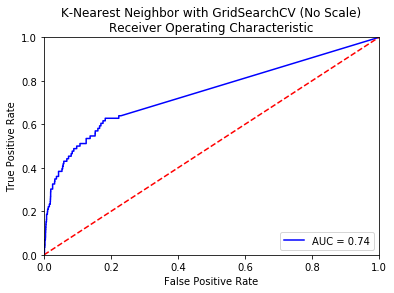
\includegraphics[width=\textwidth]{knear_gridcv_noscaling_auc.png}
         \caption{AUC graph}
         \label{fig:knear_gridcv_noscale_auc}
\end{subfigure}
\caption{Results of the K-Nearest Neighbor with GridSearchCV (without scaling).}
\label{fig:knear_gridcv_noscale}
\end{figure}

\item \textbf{K-Nearest Neighbor with GridSearchCV (Scaling):}\\
%
\textbf{Scaling:} The independent variables (X\_train and X\_test) are scaled into the range such that the range is now between 0 and 1
using the min-max scaler.
The scaling gives significant accuracy improvement than the model without scaling as in Figure \ref{fig:scalingeffect}.\\
\begin{figure}[h]
\centering 
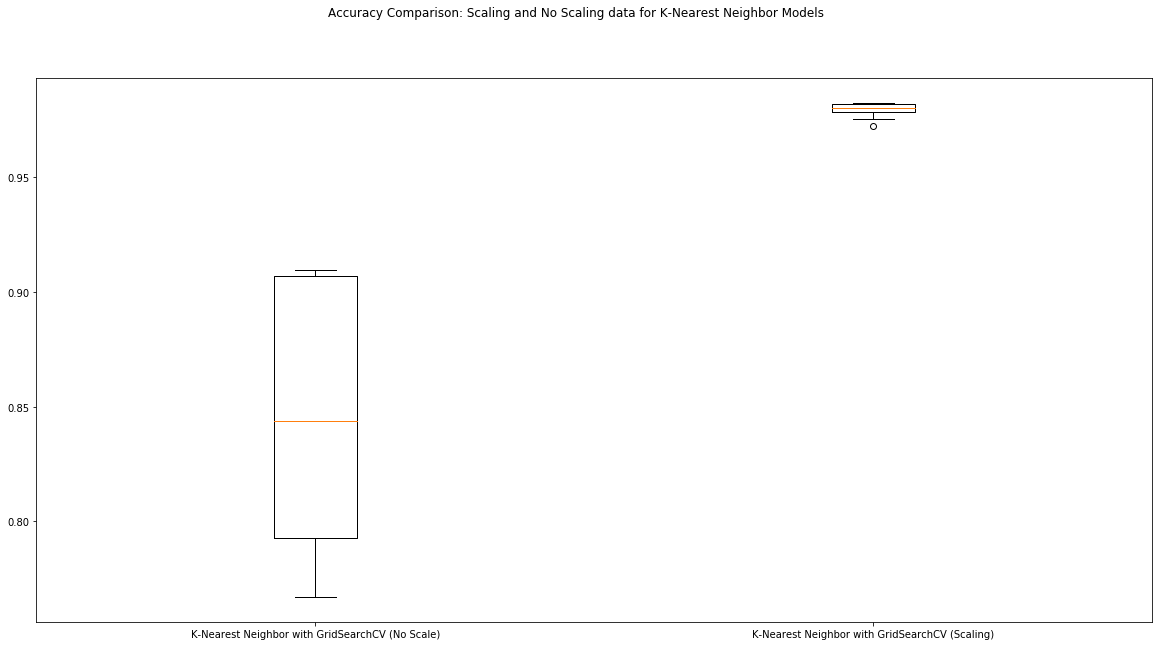
\includegraphics[scale=0.3]{knear_scaling_diff.png}
\caption{The effects of scaling in K-Nearest Neighbor Models (Scaling Before vs. After).}
  \label{fig:scalingeffect}
\end{figure}

%
Figure \ref{fig:knear_gridcv} presents 
the results of K-Nearest Neighbor using the scaling with Grid Search Cross Validation (Stratified 5-Folds CV). The cross validated parameters are same with the K-Nearest Neighbor models without scaling.
%
Here is the best parameters for the K-Nearest Neighbor: 
\{'metric': 'manhattan', 'n\_neighbors': 19, 'weights': 'uniform'\}.
%
The results model evaluation are as follows:
best accuracy: 0.9728,
best roc\_auc\_score: 0.9618,
weighted avg precision: 0.9692,
weighted avg recall: 0.9728, and
weighted avg f1-score: 0.9695.
%
\begin{figure}[h]
\centering
\begin{subfigure}{0.6\textwidth}
         \centering
         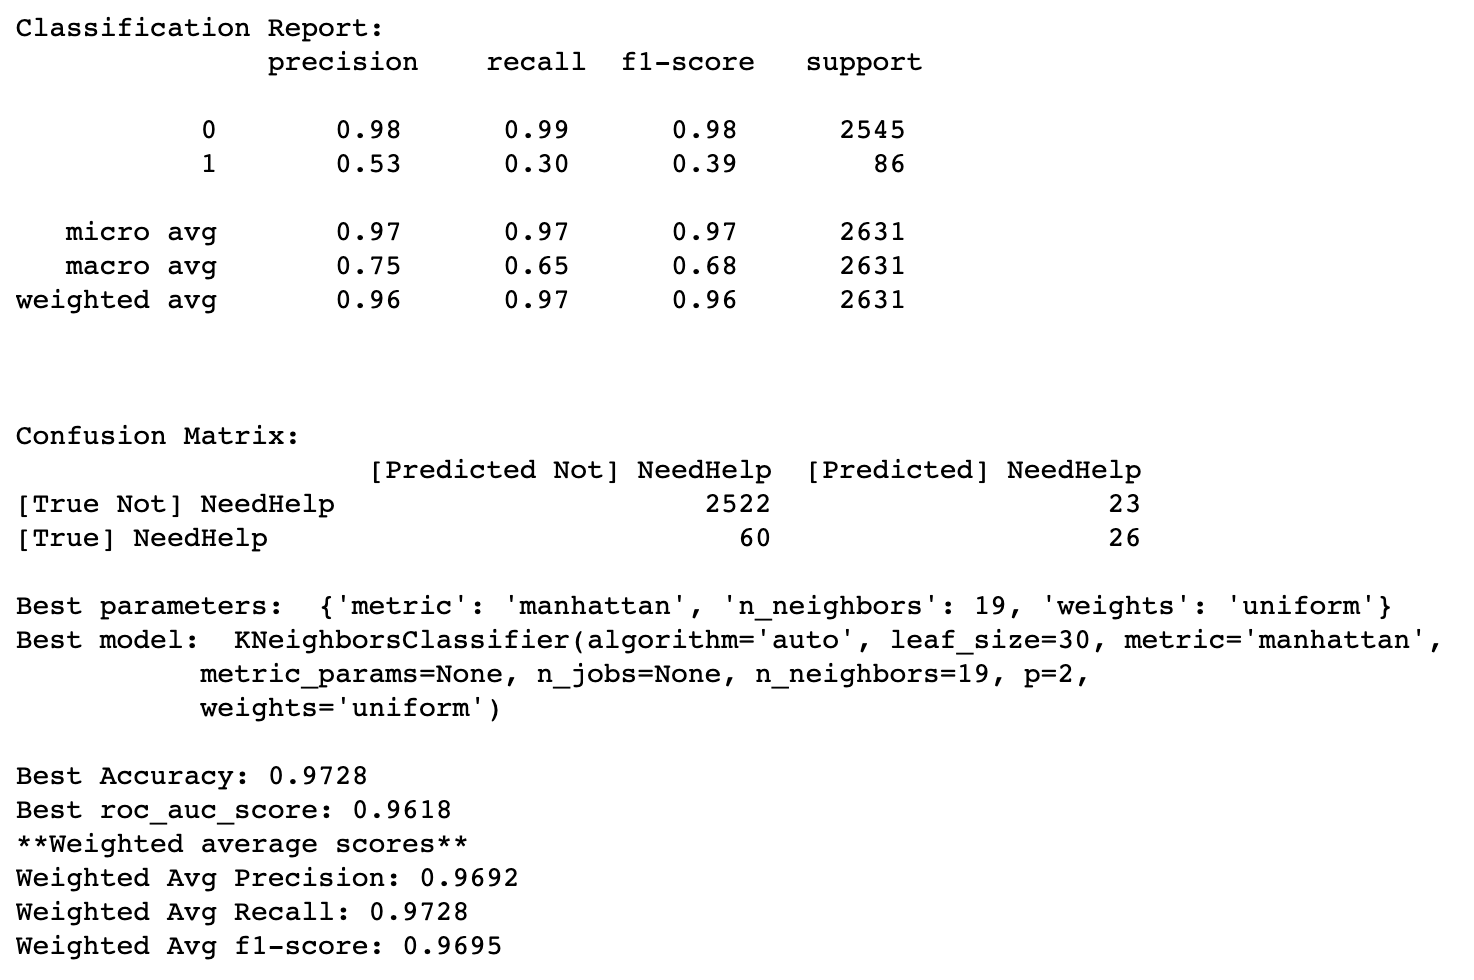
\includegraphics[width=\textwidth]{knear_gridcv.png}
         \caption{Result}
         \label{fig:knear_gridcv_report}
\end{subfigure}
\hfill
\begin{subfigure}{0.38\textwidth}
         \centering
         \includegraphics[width=\textwidth]{knear_gridcv_auc.png}
         \caption{AUC graph}
         \label{fig:knear_gridcv_auc}
\end{subfigure}
\caption{Results of the K-Nearest Neighbor with GridSearchCV (Scaling).}
\label{fig:knear_gridcv}
\end{figure}

\end{itemize}


%===================%
\subsubsection{Results of Classification:}

\begin{figure}[h!]
\centering 
\includegraphics[scale=0.35]{clf_results.png}
\caption{Boxplots of Accuracy Comparison for GridSearch CV Models.\\
Decision Tree, Random Forest Classifier, K-Nearest Neighbor (no scale), and K-Nearest Neighbor (scaling) with GridSearchCV}
  \label{fig:clf_results_gridcv}
\end{figure}

In Figure \ref{fig:clf_results_gridcv}, we have plotted the accuracy for models using the Grid Search Cross Validation. The range for each model indicates the accuracy results obtained from all parameters. 
%
\textbf{The Random Forest Classifier model has the highest accuracy.} The difference between maximum and minimum accuracy of the Random Forest Classifier is very small. 
% 
We also noted that \textbf{after applying the scaler to the K-Nearest Neighbor model, the accuracy has been significantly improved}.

Finally, 
Table \ref{table:acc_classification} shows the results of the performance for classification models. 
%
The \textbf{Random Forest Classifier with GridSearchCV worked best} with 
best accuracy: 0.9733,
best roc\_auc\_score: 0.9774,
weighted avg precision: 0.9711,
weighted avg recall: 0.9733, and
weighted avg f1-score: 0.9718.
%
The best parameters for the Random Forest Classifier model is 
\{'max\_depth': 100, 'min\_samples\_leaf': 1, 'n\_estimators': 200\}.

\begin{table}[h!]
\centering
\begin{tabular}{||c|c|c|c|c|c||}
  \hline
Model Name & accuracy & auc & precision & recall & f1\\
  \hline
Logistic Regression with Stratified 5-Folds CV &
0.9656	& 0.9656 &	0.9646 &	0.9656  &	0.9597 \\
\hline
Decision Tree with Stratified 5-Folds CV & 
0.9596	&0.7320	&0.9660	&0.9596	&0.9614\\
\hline
Decision Tree with GridSearchCV & 
0.9684	&0.9070	&0.9666	&0.9684	&0.9674\\
\hline
\cellcolor{red!25}Random Forest Classifier with GridSearchCV& \cellcolor{red!25}0.9733& \cellcolor{red!25}0.9774&  \cellcolor{red!25}0.9711& \cellcolor{red!25}	0.9733	& \cellcolor{red!25}0.9718\\
\hline
K-Nearest Neighbor with GridSearchCV (No Scale) & 
0.9650&	0.7309&	0.9556&	0.9650&	0.9526\\
\hline
\cellcolor{green!25}K-Nearest Neighbor with GridSearchCV (Scaling) & 
\cellcolor{green!25}0.9728&	\cellcolor{green!25}0.9618&	\cellcolor{green!25}0.9692&	\cellcolor{green!25}0.9728&	\cellcolor{green!25}0.9695\\
  \hline
\end{tabular}
\caption{Results for the performance of classification models.}
\label{table:acc_classification}
\end{table}



\section{Limitation and Recommendation}
\label{Limitation and Recommendation}

\paragraph*{Limitation.}

I assumed that the family incomes of students could be an important factor affecting the school performance achievements in scores. Therefore, I used the median/mean house prices from Zillow \cite{Zillow_research_data} by matching the zip codes of schools.
%
However, after analyzing in detail, I found that the range covered by postal codes is too broad, so median/mean housing prices do not properly reflect the school's family income.
%%(from GreatSchools API reference)
For example, Mission Education Center school (located in San Francisco Unified School District in San Francisco County) has the median house price of \$1,662,300 but \href{https://www.greatschools.org/california/san-francisco/6410-Mission-Education-Center/#Low-income_students}{89\% of students from low-income families}.
%
%https://www.greatschools.org/california/san-francisco/6410-Mission-Education-Center/#Low-income_students
%
%https://www.greatschools.org/california/sacramento/4771-Dyer-Kelly-Elementary-School/#Reviews
%
I should have considered another complementary variables for the family incomes of students such as ``low income family ratio".

%
The additional datasets can be considered to obtain more accurate prediction or more valuable insights. For example, we can collect the following data:
\begin{itemize}
\item Teacher demographics (from Civil Rights Data Collection)
\item School profile, school reviews, school census data, nearby schools
\end{itemize}

\paragraph*{Recommendation.}

It is obvious that that the high scores of schools are strongly correlated with the students raised in high-income families.
The students in high income families are more exposed to various learning opportunities including lessons in sports, musical instruments, arts or other activities. 
%
Learning achievement naturally leads to academic achievement, but
students who have not had the pleasure of learning may give up their academic endeavors early or even not start studying at all.

Thus, in my opinion, 
\textbf{the schools need the help}
if 
%ok
the schools have more than 73.14\% of students of low-income families, 
%ok
the house median prices are less than \$335,500 (more urgent help is needed when the house prices are when less than \$194,350), 
%
the parents who do not graduate high schools is more than 89.1\%,
%
the parents who do not graduate colleges is more than 84.9\%, or
%
the Hispanic or Black students is more than 67.2\%.
%
%
For reference, we provide the distribution graphs of important features for bottom 5\% (181 schools) and top 5\% (179 schools) performing school data in Figure \ref{fig:distribution_level1and4}. We made the above suggestions by referencing the decision trees constructed using each of important features as Figures \ref{fig:dtree_specific_features}.
%\ref{fig:dtree_specific_eco_disrate}, 
%\ref{fig:dtree_specific_house},
%\ref{fig:dtree_specific_nocollege},
%\ref{fig:dtree_specific_nohigh},
%and \ref{fig:dtree_specific_hispanic}.

I examined the Google reviews written by the students who attended the bottom 5\% schools, and consistently noticed the following  comments:
\begin{quote}
\textit{``The class is boring. There are no effective approach for homework. Teachers are not effective in teaching. The teachers don't seem interested in the students succeed.''}
\end{quote}
%
To increase academic achievement effectively, 
more budgets need to be allocated to schools to hire
teachers or staffs for providing the 1 to 1 interaction or private tutoring. 
These schools need more money to purchase academic applications and electronic devices that help students learn in the fun and independent environment.

%============
\begin{figure}[h!]
\centering 
\includegraphics[scale=0.38]{distribution_level1vs4.png}
\caption{Distribution of important features for bottom 5\% and top 5\% (Level 1 vs Level 4).\\
X-axis: 1) House median(\$), 2) Parent Education: Graduates(\%), 3) Parent Education: Not High School Graduates(\%), 4) Ethnicity: Hispanic and Black(\%), and 5) Economically Disadvantaged(\%).}
  \label{fig:distribution_level1and4}
\end{figure}
%============
\begin{figure}[h!]
\centering
\begin{subfigure}{0.4\textwidth}
         \centering
         \includegraphics[width=\textwidth]{recom_economic_dis_rate.png}
         \caption{Percentage of economically disadvantaged students}
         \label{fig:dtree_specific_eco_disrate}
\end{subfigure}
\hfill
\begin{subfigure}{0.55\textwidth}
         \centering
         \includegraphics[width=\textwidth]{recom_house_median.png}
         \caption{House median prices}
         \label{fig:dtree_specific_house}
\end{subfigure}
\hfill
\begin{subfigure}{0.45\textwidth}
         \centering
         \includegraphics[width=\textwidth]{recom_edu_notcollege.png}
         \caption{Percentage of students whose parents do not graduated the colleges}
         \label{fig:dtree_specific_nocollege}
\end{subfigure}
\hfill
\begin{subfigure}{0.5\textwidth}
         \centering
         \includegraphics[width=\textwidth]{recom_edu_nothigh.png}
         \caption{Percentage of students whose parents do not graduated the high schools}
         \label{fig:dtree_specific_noghigh}
\end{subfigure}
\hfill
\begin{subfigure}{0.7\textwidth}
         \centering
         \includegraphics[width=\textwidth]{recom_hispanic.png}
         \caption{Percentage of Hispanic and Black students}
         \label{fig:dtree_specific_hispanic}
\end{subfigure}
\caption{Decision Trees for each of important feature using the bottom 5\% and top 5\% performing school data.}
\label{fig:dtree_specific_features}
\end{figure}
%============
%============
%\begin{figure}[h]
%\centering 
%\includegraphics[scale=0.2]{recom_economic_dis_rate.png}
%\caption{Decision Tree for the ``percentage of economically disadvantaged students" (using the bottom 5\% and top 5\% performing school data).}
%  \label{fig:dtree_specific_eco_disrate}
%\end{figure}
%
%\begin{figure}[h]
%\centering 
%\includegraphics[scale=0.2]{recom_house_median.png}
%\caption{Decision Tree for the ``house median prices" (using the bottom 5\% and top 5\% performing school data).}
%  \label{fig:dtree_specific_house}
%\end{figure}
%
%\begin{figure}[h]
%\centering 
%\includegraphics[scale=0.2]{recom_edu_notcollege.png}
%\caption{Decision Tree for the ``percentage of students whose parents do not graduated the colleges" (using the bottom 5\% and top 5\% performing school data).}
%  \label{fig:dtree_specific_nocollege}
%\end{figure}
%
%\begin{figure}[h]
%\centering 
%\includegraphics[scale=0.2]{recom_edu_nothigh.png}
%\caption{Decision Tree for the ``percentage of students whose parents do not graduated the high schools" (using the bottom 5\% and top 5\% performing school data).}
%  \label{fig:dtree_specific_nohigh}
%\end{figure}
%
%\begin{figure}[h]
%\centering 
%\includegraphics[scale=0.2]{recom_hispanic.png}
%\caption{Decision Tree for the ``percentage of Hispanic and Black students" (using the bottom 5\% and top 5\% performing school data).}
%  \label{fig:dtree_specific_hispanic}
%\end{figure}
%============

\section{Conclusion and Future Work}

We have analyzed the CAASPP score data 
to help predict and find the inferior groups of schools that indeed need help.

%should be included in project1.md (2019/6/21)
\paragraph*{Data Wrangling.} In the data wrangling,
we performed data cleaning, fixing missing values, and adding new columns.
%
Missing values are imputed using the statistics of the \textit{mean} of each column in which the missing values are located.
%
We add the new variables by manipulating or merging existing variables to tell new insights or to reduce the dimensionality.

\paragraph*{Exploratory Data Analysis.}
In the data visualization, we investigated the three research questions. 
%RQ1
To answer how the students are different in achievement levels, we provided the \textbf{bar plots for the comparison for each category of gender, ethnicity, English-language fluency, economic status, disability status, and parent educations}.
For utilizing the advanced features, we also used the Plotly libraries for drawing interactive graphs.
The major finding are as follows:
\begin{itemize}
	\item Female students exceed male students in English, while male students exceed female students in Mathematics.
\item Asian students achieve the best performance, while Black or African American and American Indian or Alaska Native students achieve the lowest performance in both English and mathematics.
\item Initial fluent English proficient students achieve the best performance in both English and mathematics.
\item The economically disadvantaged students have much more difficulties than not-economically disadvantaged students.
\item Only the small number of students with disabilities could achieve the best performance.
\item The higher the level of parental education, the higher the achievement of students.
\end{itemize}
%RQ2
To find the features in the top and bottom performance groups,
we compared the best and worst 10\% performing counties (10\% out of 58 = 5 counties) using the bar plots. 
We found that the test performance is closely related
to the economic capabilities of the family to which the student belongs.
%
We could observe that Hispanic and Latino students are far more likely to be in the worst performing group than the best performing group.
%
By contrast, Asian and white students are more likely to be in the best performing group than the worst performing group.
%RQ3 
For the last, to investigate how house prices are correlated to the exceeded scores or inferior scores, we analyzed the correlations using scatterplots. We observed the strong positive correlations between the ``Percentage of Standard Exceeded” and the house prices whereas the strong negative correlations between the``Percentage of Standard Not Met” and the house prices.

%
In the exploratory data analysis,
we used the inferential statistics to identify significant features.
%
%We preprocessed the data by transforming data into school levels.
%
A significant number of features could be redundant and irrelevant, therefore it is important to apply feature selection/dimension reduction. We performed the statistical hypothesis testing, correlation test, and feature selection for getting rid of the student group information for generating less number of features.
%
First, we test whether the means of two independent samples are significantly different and eliminated or merged the weak affecting
student group indicators.
%
Next, for correlation analysis, we used the matrix with Heatmap, Pearson's correlation coefficient, and Spearman's rank correlation methods and found the meaningful strong relationships between pairs of features (e.g., house prices and high scores, advanced education of students' parents and high scores). 
%
For the last, for the feature selection, we used the univariate selection and feature importance techniques and could obtain a score for each feature of the data and prioritize the in the order of importance.

\paragraph*{Models.}
The aim is to predict the inferior scores of schools. We used the supervised machine learning  algorithms including the regression and classification to build predictive models.
%======
The regression algorithm predicts the percentage of students who do not meet the standard. The classification algorithm predicts if the schools ``need help" or "do not need help". 
%
We set the ``need help" schools that has more than ``80\% of the standard not met" students (312 out of 8,786 schools).
%
We tried various machine learning techniques to pick the one which performs best.
%
For regression, out of 5 different models, we obtained the best regression model using the random forest regressor with 10 folds cross validation
with the accuracy of RMSE 10.77, MAE 7.69, and R$^{2}$ 0.68.
%
For classification, we tried to solve the class imbalanced problems using the Stratified K-fold cross validation and the weighted evaluation metrics to reflect the mass of the classes. In addition, we scaled the training data and significantly improved the accuracy of the K-Nearest Neighbor algorithm.
%
As a result, out of 5 different models, we obtained the best classification model using the random forest classifier based on grid search cross validation (three parameters each of three values)
with the accuracy 0.97, AUC 0.98, precision 0.97, recall 0.97, and f1-score 0.97. 

%===============================
For the future work,
to identify the factors that could effectively improve the scores, we will investigate the scores of the 5 consecutive years (2014 to 2018 available in \cite{california_dep_education}). 
%
We expect to find the important features on the schools in which the scores have been dramatically improved.
%

For the final comment, I hope this school score prediction analysis could be a little help to administrators to the California state departments of education, teachers and parents to broadening educational opportunities.

I give my special thanks to Tony Baek who has been my mentor for completing this project.

\newpage
\bibliography{scibib}
\bibliographystyle{Science}

%\bibliography{arhan}
%\bibliographystyle{IEEEtran.cls}

\end{document}


















